%% The following is a directive for TeXShop to indicate the main file
%%!TEX root = diss.tex

\chapter{A Mapping of 3D Reconstruction}
\label{ch:3DRecon_Mapping}
Most vision work focuses on developing algorithmic novelties, and as we have mentioned, very few investigate the rigorous conditions under which the algorithms themselves work. Thus, this knowledge is only known empirically, without a rigorous definition of the application domain or problem conditions. This relation between problem space and algorithms (termed as \textit{mapping}) is one of the key components of the interpreter, and is responsible for selecting one of the best possible algorithms based on described problem condition. The mapping is essentially a look-up table that returns a list of successful algorithms given a problem condition. This section builds upon the 3D description proposed in Chapter~\ref{ch:3DRecon_Desc}, and attempts to find the problem conditions surrounding each algorithm empirically. 

To achieve this goal, we need a dataset to evaluate the performance of each algorithm under varied problem conditions, which is not available since most 3D benchmarks, to the best of our knowledge, focus on one specific class of algorithms. For example, the Middlebury dataset targets MVS algorithms~\cite{seitz2006comparison}, and the `DiLiGenT' dataset targets Photometric Stereo algorithms~\cite{shi2016benchmark}. This makes such benchmarks only suitable for evaluation of within-category algorithms. Besides, there are no datasets with objects that cover a range of properties of materials and geometry. The reason for the lack of such a dataset is that it is practically impossible to change one property, \eg surface texture, material, and so on, while fixing others when creating a real-world dataset.

In response to these challenges, we use synthetic datasets created by phiyical-based rendering software (Blender), to evaluate the 3D reconstruction algorithms. Our dataset includes a collection of images of a scene under different materials and lighting conditions. The camera/projector's intrinsic and extrinsic parameters are computed directly from the configurations of the synthetic setup, and the ground truth, including the 3D model point cloud and normal map, are generated directly from Blender.

\section{Synthetic setup}
We use Blender's physical-based rendering engine, Cycles, to generate the synthetic datasets. For each technique, the configuration of the camera remains fixed. The image resolution is 1280$\times$720, with a focal length of $35mm$ or $1400pix$. The synthetic setups are shown in Table~\ref{tab:synth_setup}, and some example synthetic images generated using the setups are shown in Figure~\ref{fig:synth_setup}.
\begin{table}[!htbp]
\centering
\begin{tabular}{lll}
\toprule
Method & Hardware number & Arrangement\\
\midrule
MVS & 41 camera & 5 rings, each having 1, 8, 8, 12, 12 camera\\
PS & 1 camera+25 lights & 4 rings, each having 1, 8, 8, 8, 8 light sources\\
SL & 1 camera\&projector & baseline angle: $10^\circ$\\
\bottomrule
\end{tabular}
\caption{Summary of synthetic setups.}
\label{tab:synth_setup}
\end{table}

\begin{figure*}[!htbp]
\centering
\begin{tabular}{ll}
Texture & \raisebox{-.5\height}{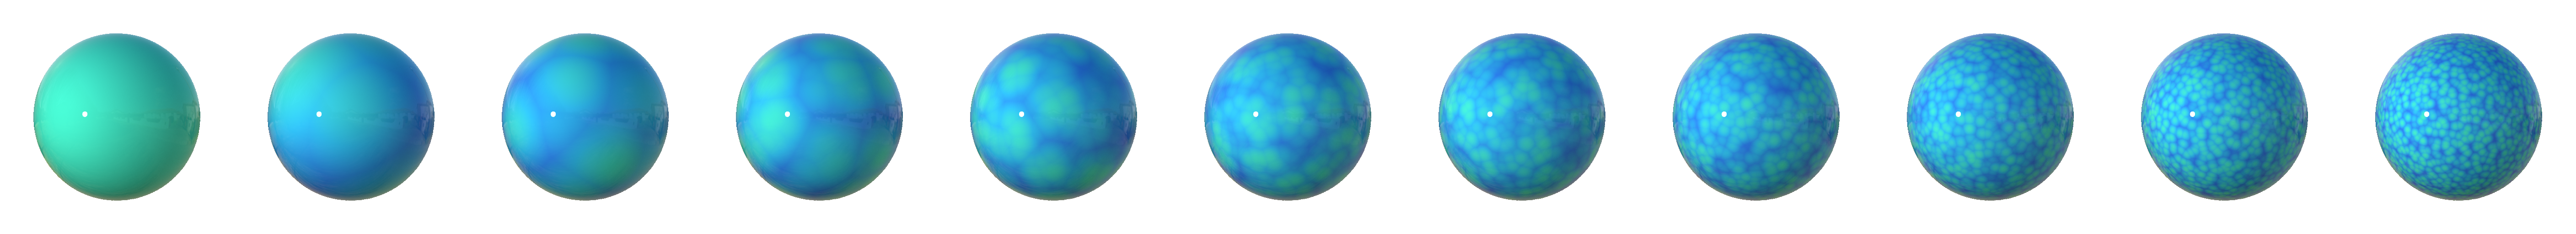
\includegraphics[width=0.8\textwidth]{img/mapping/setup/tex.png}}\\
Albedo & \raisebox{-.5\height}{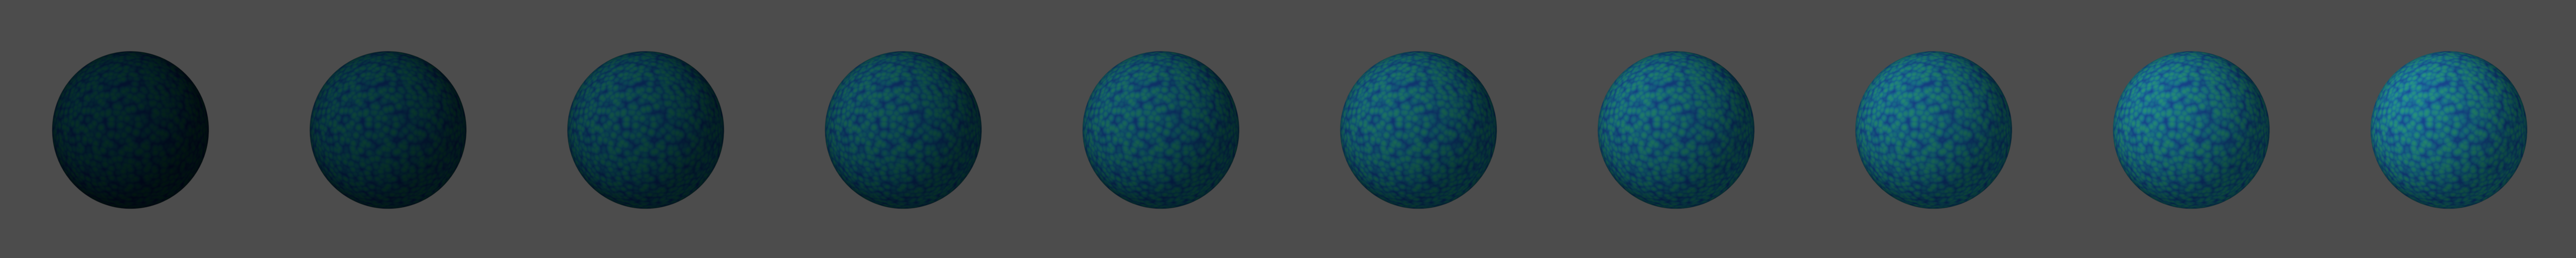
\includegraphics[width=0.8\textwidth]{img/mapping/setup/alb.png}}\\
Specular & \raisebox{-.5\height}{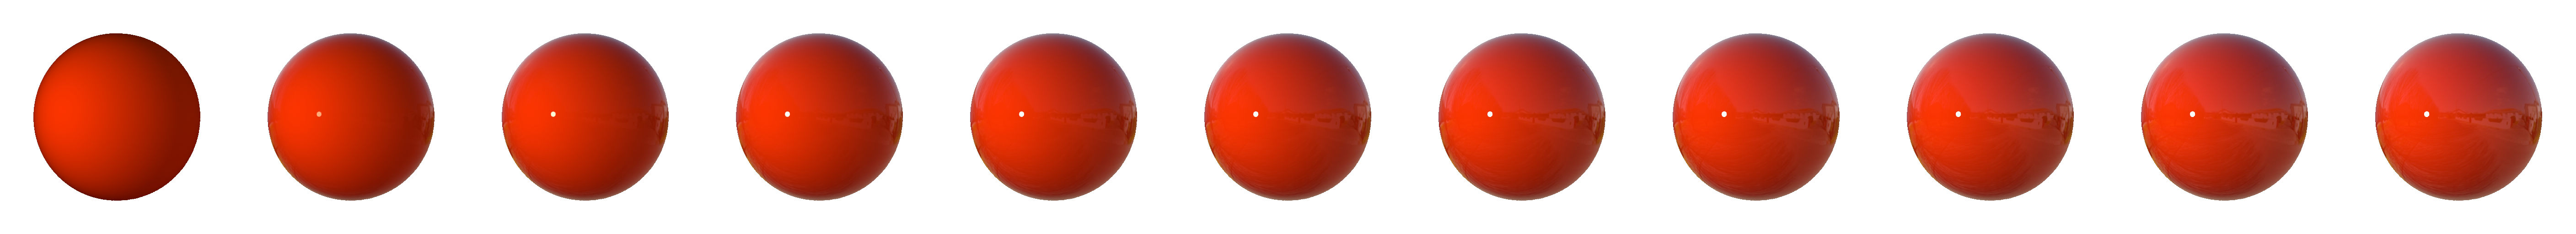
\includegraphics[width=0.8\textwidth]{img/mapping/setup/spec.png}}\\
Roughness & \raisebox{-.5\height}{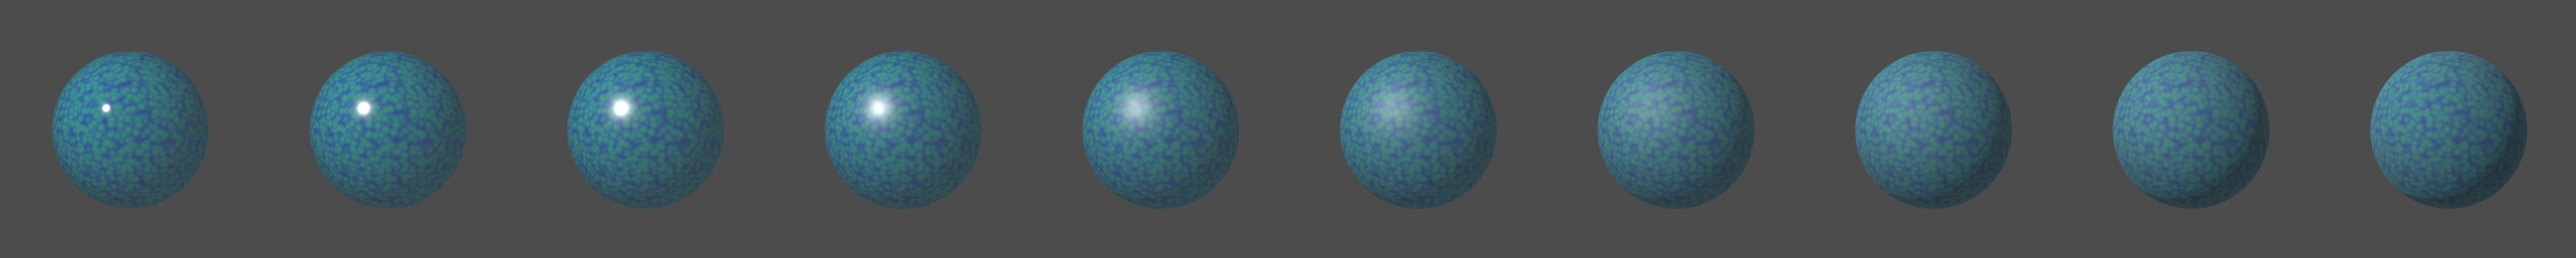
\includegraphics[width=0.8\textwidth]{img/mapping/setup/rough.png}}
\end{tabular}
\caption{Example synthetic images. The value of each property ranges from 0.1 to 1.}
\label{fig:synth_setup}
\end{figure*}

% For the Multi-View Stereo setup, there are five rings of cameras, of which the elevation angles are $15^\circ$, $30^\circ$, $45^\circ$, $60^\circ$, $90^\circ$. The between-angles of two neighbouring cameras are $30^\circ$, $30^\circ$, $45^\circ$, $45^\circ$, and $360^\circ$. Thus, there are in total $12+12+8+8+1=41$ cameras.

% For the Photometric Stereo setup, since increasing the number of images is only important up to a point, the experimental results showed that most algorithms reaches their optimum when 15 images are used~\cite{Berkiten:2016:ARB}. To strike a balance between algorithm performance and rendering time, we use 25 light sources, which are distributed on four rings with elevation angle of $90^\circ$, $85^\circ$, $60^\circ$, and $45^\circ$. The azimuth angle between two neighbouring light sources is $45^\circ$. Thus, the total number of images is $1+8*3=25$.

% For the Structured Light setup, the baseline angle between the camera and the projector is $10^\circ$. The resolution of the projector is $1024\times768$, thus 10 Gray code patterns are needed. To counter the effect of inter-reflection, each pattern and its inverse are projected, which descreases sensitivity to scattered light. Two additional image with lights on and off are generated to help the decoding process. Thus the total number of images is $(10+10)*2+2=42$.
% \begin{figure}[!htbp]
% \centering
% \begin{tabular}{ccc}
% 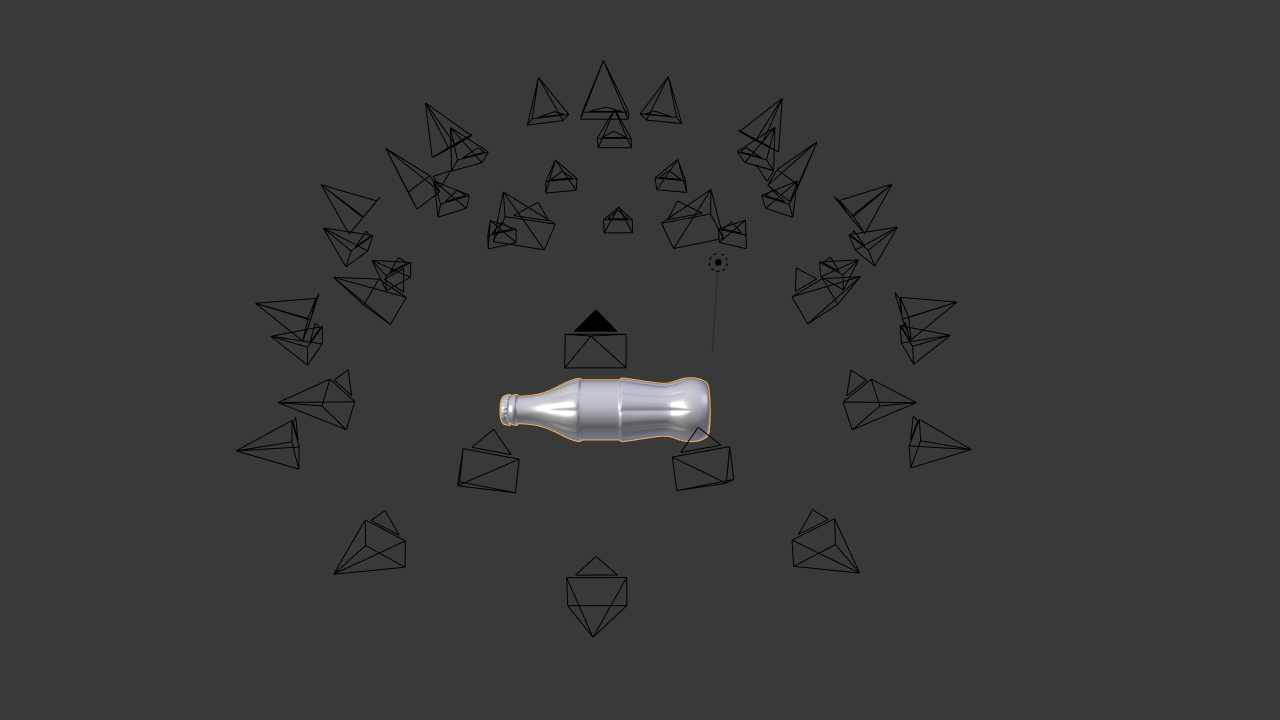
\includegraphics[width=0.3\textwidth]{mapping/setup/mvs_setup} &
% 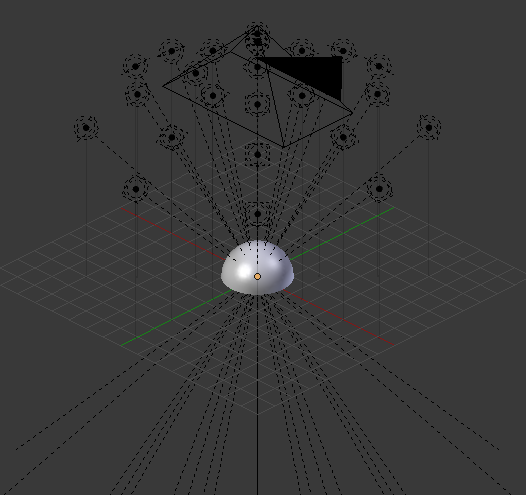
\includegraphics[width=0.3\textwidth]{mapping/setup/ps_setup} &
% 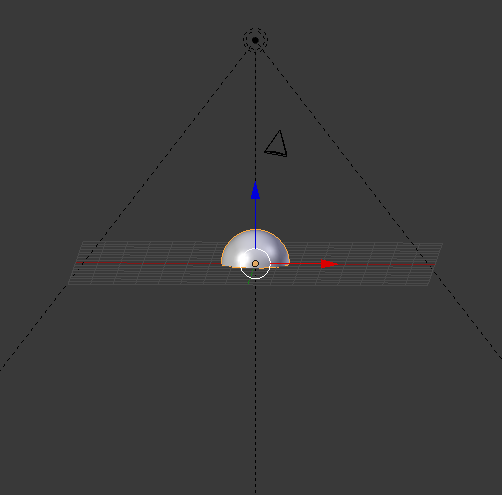
\includegraphics[width=0.3\textwidth]{mapping/setup/sl_setup}\\
% MVS & PS & SL\\
% \end{tabular}
% \caption{Setups of the syntheic dataset}
% \label{fig:setup}
% \end{figure}

% \section{Structure of Datasets}
% All synthetic datasets used in this thesis share the similar structure, as shown in Figure~\ref{fig:dataset_structure}. \textit{Prop Comb} represents one combination of properties, which consists of no less than two properties. For instance, \textit{texture and albedo}, or \textit{albedo, and specularity}. Note that the diretory structure of PS and SL is the same as that of MVS.
% Due to the number of properties and levels for each property, it would be unrealistic to render all their combinations. For instance, if there are $N$ properties and each is discretized into $L$ levels, the number of different combinations is $L^N$, and for each combination, there are in total $41+25+42=108$ images to render. Therefore, we take another approach: 1) we investigate the \textit{effective problem domain} which consists of only the \textit{effective} and \textit{dependent} properties; 2) we generate synthetic images for the \textit{effective} and \textit{dependent} properties and all of their combinations. The structure of the dataset is as follows:
% \begin{figure}[!htbp]
% \centering
% 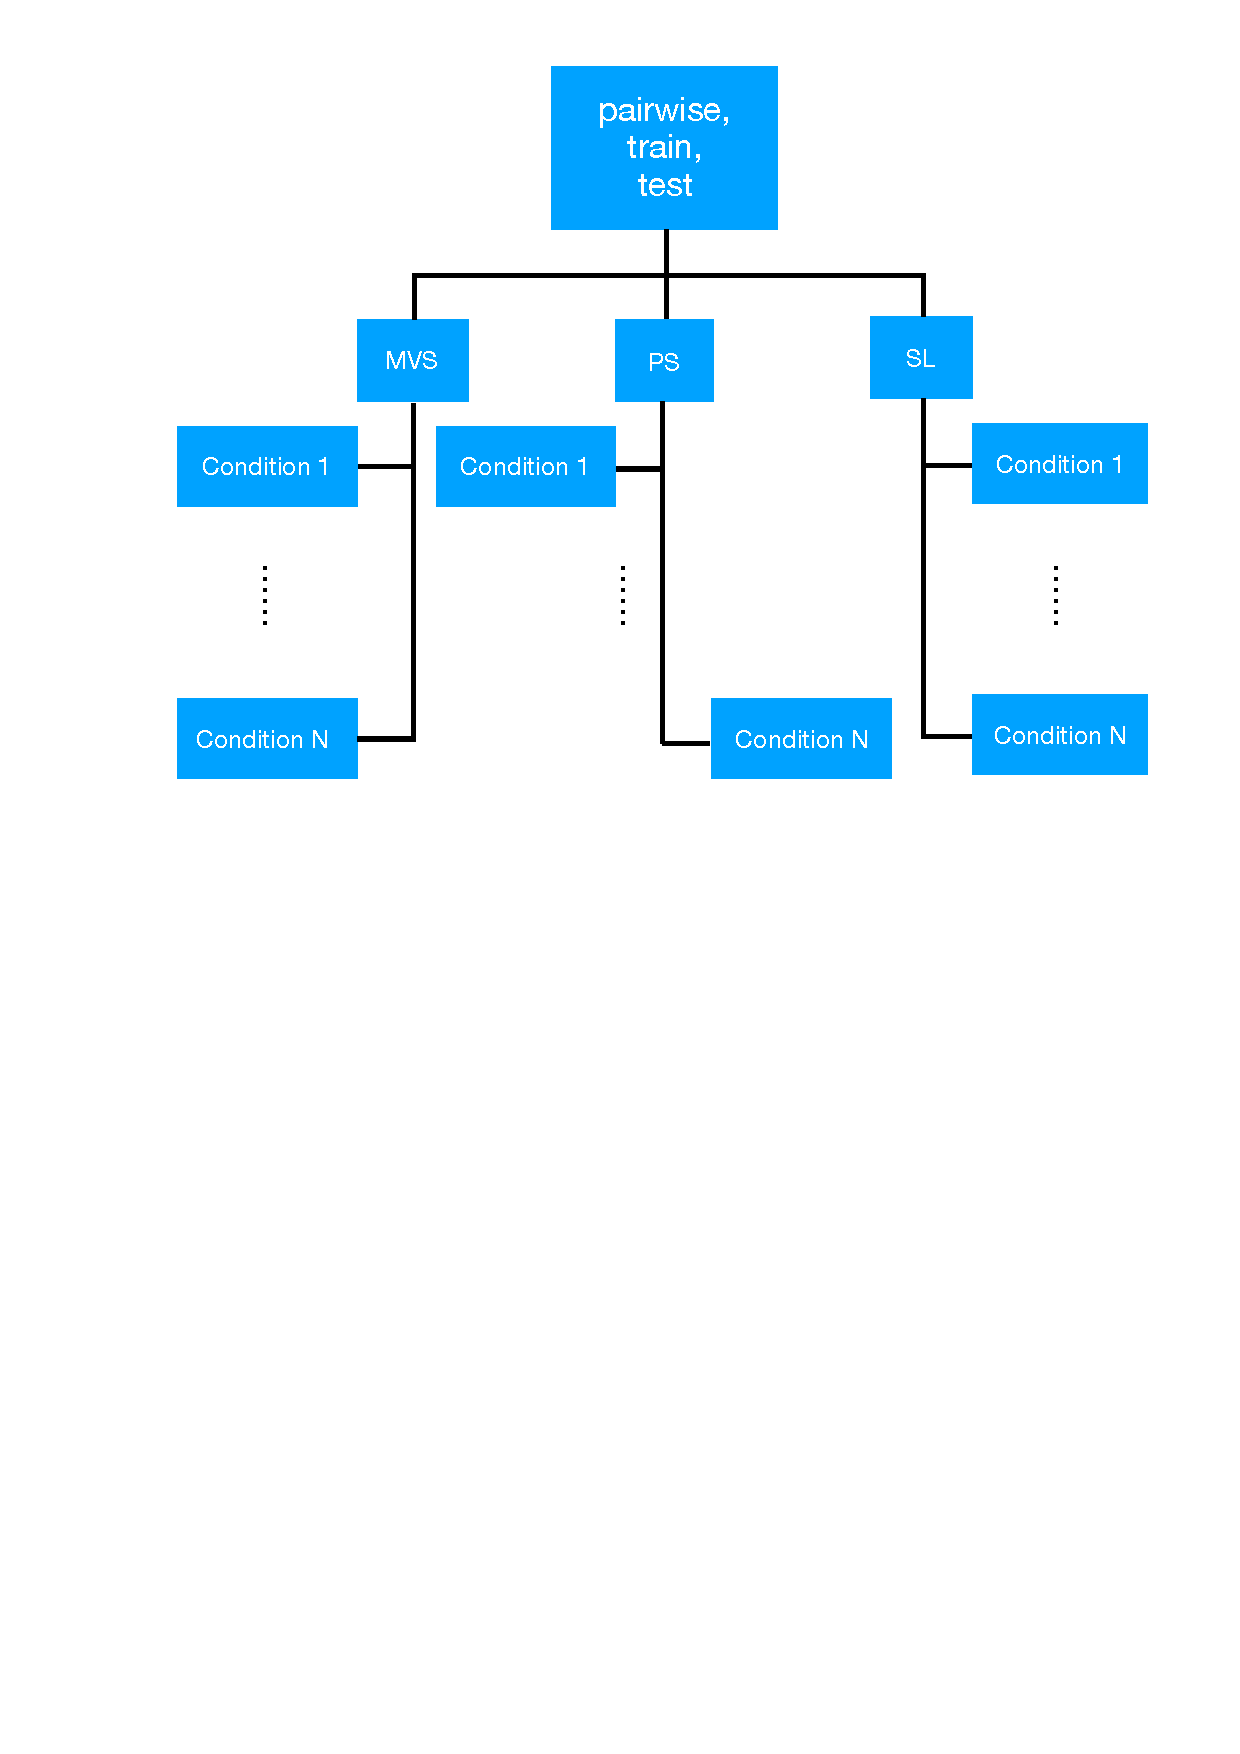
\includegraphics[width=0.6\textwidth]{mapping/dataset_structure}
% \caption{Structure of the synthetic dataset.}
% \label{fig:dataset_structure}
% \end{figure}

\section{Selected and baseline methods}
We have selected one representative algorithm from three major classes of algorithms presented in Chapter~\ref{ch:3DRecon_ProbSpace}: the PMVS proposed in~\cite{furukawa2010accurate}, the example-based Photometric Stereo proposed in~\cite{hertzmann2005example}, and the Gray-code Structured Light technique. See Table~\ref{tab:selected_algos} for a summary of the selected algorithms. The current implementation of SL projects both column and row patterns, and depth values are computed using these two kinds of patterns individually. A depth consistency step is performed to reject erroneous triangulations.
\begin{table}[!htbp]
\centering
\begin{tabular}{l|l}
\toprule
Technique & Summary\\
\midrule
PMVS & Patch-based, seed points propagation MVS.\\
EPS & Example-based Photometric Stereo.\\
GSL & Gray code Structured Light technique.\\
\midrule
VH & Volumetric Visual Hull.\\
LLS-PS & Linear least squares Photometric Stereo.\\
\bottomrule
\end{tabular}
\caption{Summary of the selected and baseline algorithms for the interface, and the corresponding working conditions in theory.}
\label{tab:selected_algos}
\end{table}

% \section{Baseline}
% \begin{table}[!htbp]
% \centering
% \begin{tabular}{c|c|c|c|c}
% \toprule
% Technique & Texture & Albedeo & Specular & Roughness\\
% \midrule
% \multicolumn{5}{l}{VH: volumetric Visual Hull}\\
% \midrule
% VH & - & - & - & -\\
% \midrule
% \multicolumn{5}{l}{LLS-PS: linear least squares Photometric Stereo.}\\
% \midrule
% LLS-PS & - & High & Low & High\\
% \bottomrule
% \end{tabular}
% \caption{Summary of the baseline algorithms for the framework, and the corresponding working conditions in theory.}
% \label{tab:selected_baseline_algos}
% \end{table}
We use two baseline approaches to compare our results: Visual Hull and a simple linear least squares based Photometric Stereo (LLS-PS). We use Visual Hull since it works relatively well as long as the silhouette of the object can be reliably extracted, thus being insensitive to material properties. In addition, the true scene is always enclosed by the reconstruction result, so the outcome is always predictable. We use LLS-PS to evaluate Photometric Stereo algorithms. However, there is currently no such PS algorithms that work reasonably well under a variety of conditions. Thus, we run this baseline algorithm under the optimal condition to ensure a best possible result.

\section{Quantitative measures}
We use the metrics proposed in \cite{seitz2006comparison} to evaluate MVS and SL algorithms. More specifically, we compute the accuracy and completeness of the reconstruction. For accuracy, the distance between the points in the reconstruction $R$ and the nearest points on ground truth $G$ is computed, and the distance $d$ such that $X\%$ of the points on $R$ are within distance $d$ of $G$ is considered as accuracy. A reasonable $d$ value is between $[3, 5]mm$, and $X$ is set as $95$. The lower the accuracy value, the better the reconstruction result. For completeness, we compute the distance from $G$ to $R$. Intuitively, points on $G$ are not ``covered'' if no suitable nearest points on $R$ are found. A more practical approach computes the fraction of points of $G$ that are within an allowable distance $d$ of $R$. Note that as the accuracy improves, the ``accuracy value'' goes down, whereas as the completeness improves, the ``completeness value'' goes up.

For photometric stereo, depth information is lost since only one viewpoint is used. Thus, the previous metrics are not applicable. Here we employ another evaluation criteria that is widely adopted, which is based on the statistics of angular error. For each pixel, the angular error is calculated as the angle between the estimated and ground truth normal, \ie $arccos$($n_g^T n$), where $n_g$ and $n$ are the ground truth and estimated normals respectively. In addition to the mean angular error, we also calculate the standard deviation, minimum, maximum, median, first quartile, and third quartile of angular errors for each estimated normal map.

% \subsection{Criteria}
% We compare the quantitative measures of a result to those of the baseline method to determine if it is a successful reconstruction. The following rules determines if a specific algorithm returns a successful reconstruction.

% For results of MVS and SL, we use both accuracy and completeness to determine if a result is successful. However, methods that return accurate results do not necessarily produce complete results. Thus, we consider a result successful if the accuracy is better while completeness is comparable to that of the baseline.

% For results of PS algorithms, we use the central value, variation, and skewness of angular error to determine if a result if successful. The rationale is explained below:

% \subsubsection{Measures of Central Tendency}
% Mean and median are both valid measures of central tendency, but as the skewness increases, the mean is dragged in the direction of the skew. As a result, the median is generally considered to be a better representative of the central location of the data. The more skewed the distribution, the greater the difference between the median and mean, and the greater the emphasis should be placed on using the median as opposed to the mean.

% \subsubsection{Variation}
% The variation of the angular error is measured by both \textit{interquatile range} ($Q_3 - Q_1$) and \textit{standard deviation} ($std$).
  
% \subsubsection{Skewness (right/positive-skewness)}
% The normal estimation becomes worse as the difference between mean and median increases. This can be explained as follows: assuming the angular error follows a Gaussian distrubtion, then mean and median are close when the normals are reliably estimated. However, if normals are poorly recovered, the mean would increase since larger angular errors exist, while the median would change far less since only a small amount of pixels are poorly estimated. Thus, the difference between mean and median is a good indicator of the quality of normal estimation.

\section{Main effects and interactions of properties}
The greatest challenge in constructing a mapping from problem space to algorithms is the large variations in shapes and material properties, which results in a problem space that is too large to cope with. Suppose there are $N$ properties, each with $L$ discrete levels, then there are in total $L^N$ different problem conditions. Thus, the first step, discussed in Section~\ref{sec:mvs_epd},~\ref{sec:ps_epd},~\ref{sec:sl_epd}, is to reduce the dimensions of problem space by discovering the properties that have effects on performance of algorithms.

This study is a $3\times 3$ factorial design with two properties (factors), each with three levels, \ie low (0.2), medium (0.5), and high (0.8). We are interested in one-way interaction (\textit{main effect}) and two-way interaction of the properties (factors).  A \textit{main effect} is the effect of one of the independent variables on the dependent variable, ignoring the effects of all other independent variables. A statistical interaction occurs when the effect of one independent variable on the dependent variable changes depending on the level of another independent variable. In our current design, this is equivalent to asking whether the effect of property $i$ changes depending on property $j$, where $i\neq j, i, j\in\{1, 2, 3, 4\}$. To determine if this is the case, we need to look at the \textit{simple main effects}: the main effect of one independent variable (e.g., property $i$) at each level of another independent variable (e.g., property $j$). The easiest way to communicate an interaction is to discuss it in terms of the \textit{simple main effects}. Describe one simple main effect, then describe the other in such a way that it is clear how the two are different. We choose to interpret the main effects and interactions through figures. We choose to use heatmaps to illustrate the effects of two properties on various metrics. There is a main effect of a property if there is color variation along the corresponding axis. If color changes monotonically along the diagonal, then there is no interaction between the two properties, otherwise, there is an interaction effect. 

% A naive way of finding the \textit{effective properties} would be evaluating algorithmic performance by changing one property at a time. However, this approach ignores the dependency between properties, \ie the effect of property \textit{A} might be insignificant when property \textit{B} is absent. Thus, we investigate the pairwise relation between any two properties, thus two properties are chosen while the rest are fixed, the configurations of the problem conditions are shown in Table~\ref{tab:pairwise_prob_cond}

\begin{table}[!htbp]
  \centering
  \begin{tabular}{l*{4}{c}}
  \hline
  \textbf{Cond.} & Texture & Albedo & Specular & Roughness\\
  \hline
  \textbf{(a)} & [0.2, 0.8] & [0.2, 0.8] & 0.0 & 0.0\\
  \textbf{(b)} & [0.2, 0.8] & 0.8 & [0.2, 0.8] & 0.0\\
  \textbf{(c)} & [0.2, 0.8] & 0.8 & 0.0 & [0.2, 0.8]\\
  \textbf{(d)} & 0.8 & [0.2, 0.8] & [0.2, 0.8] & 0.0\\
  \textbf{(e)} & 0.8 & [0.2, 0.8] & 0.0 & [0.2, 0.8]\\
  \textbf{(f)} & 0.8 & 0.8 & [0.2, 0.8] & [0.2, 0.8]\\
  \hline
  \end{tabular}
  \caption{Problem conditions for establishing the \textit{effective problem domain} of all selected algorithms. For instance, cond. (a) considers texture and albedo while specularity and roughness are fixed. The value of both varying properties range from 0.2 to 0.8.}
  \label{tab:pairwise_prob_cond}
\end{table}

\subsection{Main effects and interactions: PMVS}
\label{sec:mvs_epd}
We interpret the main effects and interactions of properties on the performance of PMVS in terms of accuracy and completeness. The settings of properties are summarized in Table~\ref{tab:pairwise_prob_cond}. The performance of the algorithm in terms of two changing properties are visualized in Figure~\ref{fig:mvs_pairwise}.
\begin{figure}[!htbp]
\begin{tabular}{cc}
\includegraphics[width=0.45\textwidth]{mapping/pairwise/mvs_tex_alb} &
\includegraphics[width=0.45\textwidth]{mapping/pairwise/mvs_tex_spec}\\
(a) & (b)\\
\includegraphics[width=0.45\textwidth]{mapping/pairwise/mvs_tex_rough} &
\includegraphics[width=0.45\textwidth]{mapping/pairwise/mvs_alb_spec}\\
(c) & (d)\\
\includegraphics[width=0.45\textwidth]{mapping/pairwise/mvs_alb_rough} &
\includegraphics[width=0.45\textwidth]{mapping/pairwise/mvs_spec_rough}\\
(e) & (f)\\
\end{tabular}
\caption{Performance of PMVS under four problem conditions. For instance, (a) shows the performance under changing \textit{texture} and \textit{albedo} values, while the others are fixed. The property values are set based on settings in Table~\ref{tab:pairwise_prob_cond}.}
\label{fig:mvs_pairwise}
\end{figure}

\textbf{(a) Texture and Albedo} 
The main effects of texture and albedo on accuracy, and the main effect of albedo on completeness are not significant whereas the effect of texture on completeness is significant such that as surfaces with higher texture leads to results of higher completeness than less textured surfaces. There is not significant interaction between texture and albedo on either accuracy or completeness.

\textbf{(b) Texture and Specularity} 
The main effects of texture and specularity on both accuracy and completeness are significant such that surfaces with low texture yields lower accuracy value whereas surfaces with high texture leads to lower accuracy value. There is a significant interaction between texture and specularity on accuracy, but not the case on completeness. More specificially, specularity has no effect on accuray for lowly/highly textured surfaces whereas it has a negative effect on surfaces with medium texture. This can be explained as follows: the specular lobe can only be observed by cameras positioned and oriented towards the specular lobe, such as camera $V_2$ shown in Figure~\ref{fig:mvs_spec} (a) and (c). Cameras positioned otherwise would observe the true surface, such as camera $V_1$ shown in Figure~\ref{fig:mvs_spec} (a) and (b). The algorithm would then exploit the texture information provided by views like $V_1$, and thus would be able to reconstruct a specular surface.
\begin{figure}[!htbp]
\begin{tabular}{ccc}
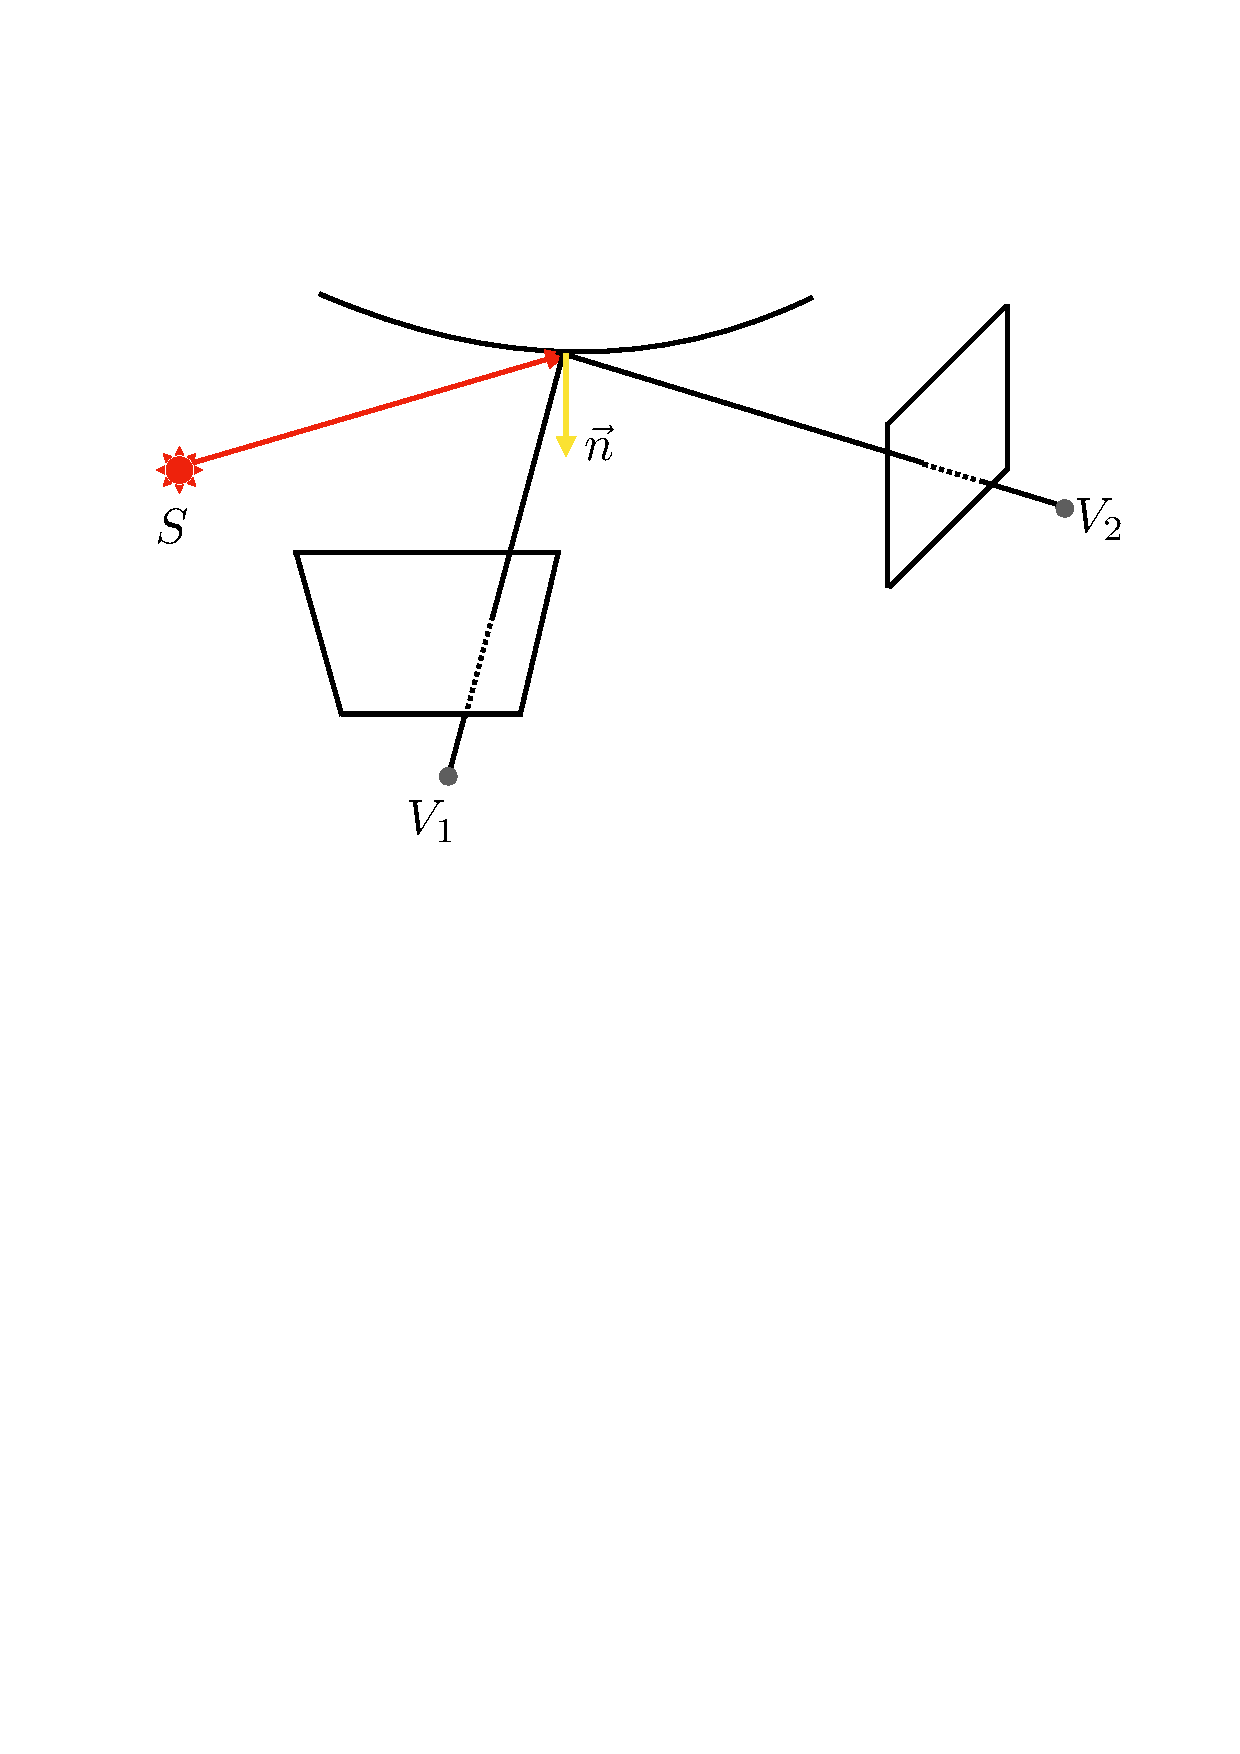
\includegraphics[width=0.3\textwidth]{mapping/mvs_spec/mvs_spec}&
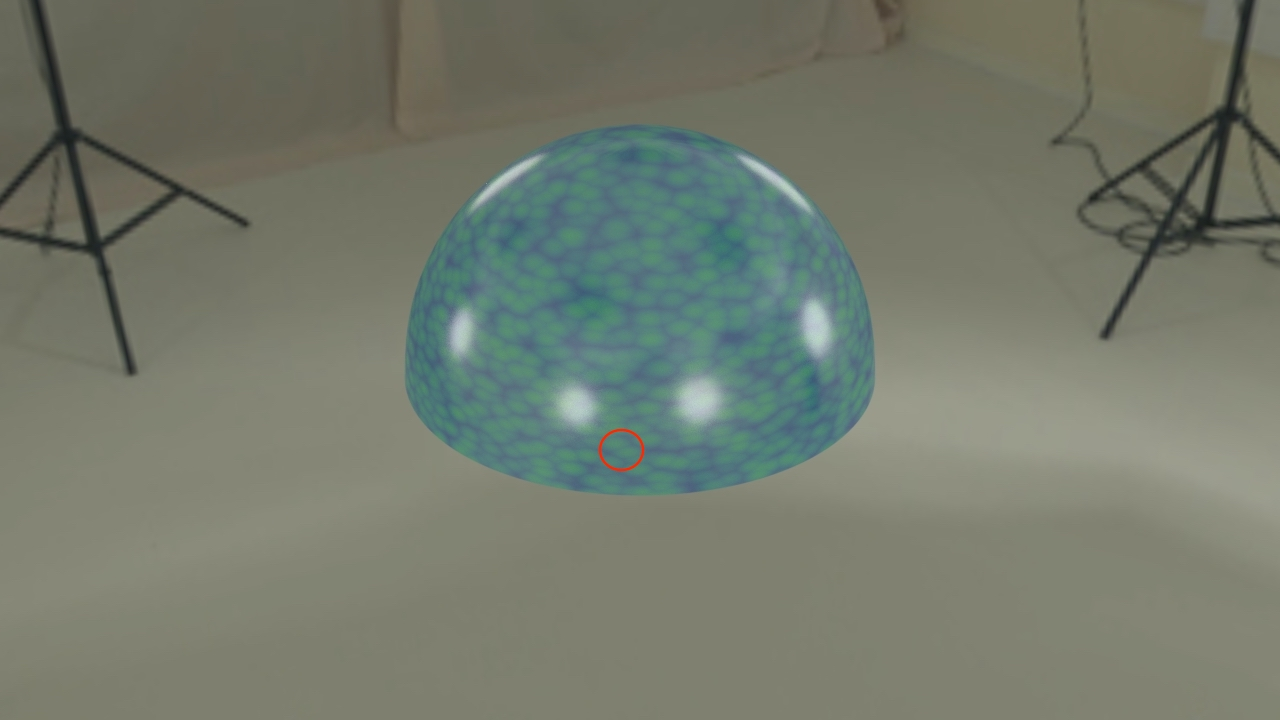
\includegraphics[width=0.3\textwidth]{mapping/mvs_spec/mvs_spec_01}&
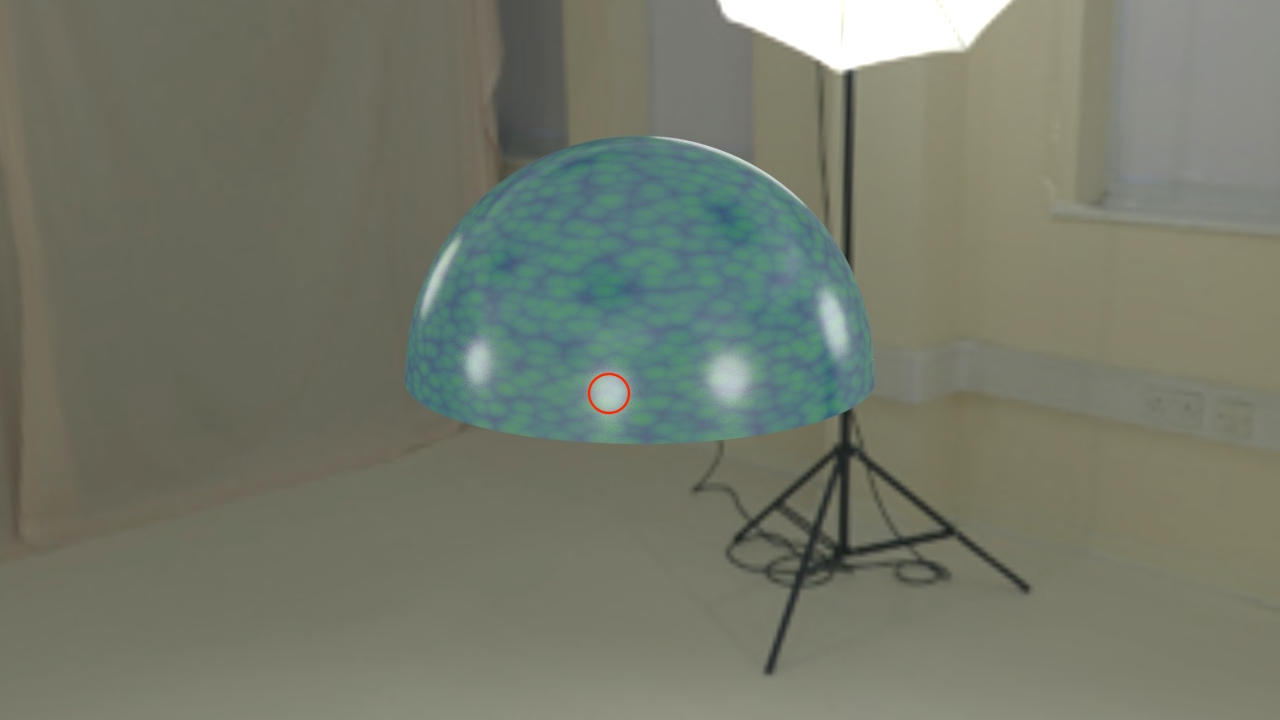
\includegraphics[width=0.3\textwidth]{mapping/mvs_spec/mvs_spec_00}\\
(a) Image formation & (b) $V_1$ & (c) $V_2$\\
\end{tabular}
\caption{(a) shows the reflection of light off a specular surface. $V_1$ received the diffuse component while $V_2$ receives the specular component. (b), (c) shows the images observed from these two views. The specular area (red circle) observed in $V_2$ is visible in $V_1$.}
\label{fig:mvs_spec}
\end{figure}

\textbf{(c) Texture and Roughness} 
The main effects of texture and roughness, and the main effect of roughness on completeness are not significant. The main effect of texture on completeness is significant such that surfaces with higher textures leads to results with higher completeness. There is no interaction effect between texture and roughness on either accuracy or completeness.

\textbf{(d) Albedo and Specularity} 
The main effects of albedo and specularity on accuracy is not significant whereas the main effects on completeness are significant such that surfaces with higher albedo or lower specularity leads to better reconstruction results in terms of completeness. There is no significant interaction effect between albedo and specularity in terms of accuracy and completeness as the value varies monotonically along the diagonal.

% albedo has a positive effect whereas specular has a negative effect on the reconstruction. Furthermore, the positive effect of albedo is more significant on a higher specular surface while the negative effect of specular is far more substantial on a lower albedo surface. This can be explained as follows: according to the energy conservation law, as the specular component increases, the diffuse component decreases, resulting in a less discernible diffuse area. See Figure~\ref{fig:mvs_alb_spec} (a)-(c). Increasing the diffuse albedo can counteract the effect of specularity and make the texture visible again. See Figure~\ref{fig:mvs_alb_spec} (d)-(f).
% \begin{figure}[!htbp]
% \centering
% \begin{tabular}{ccc}
% 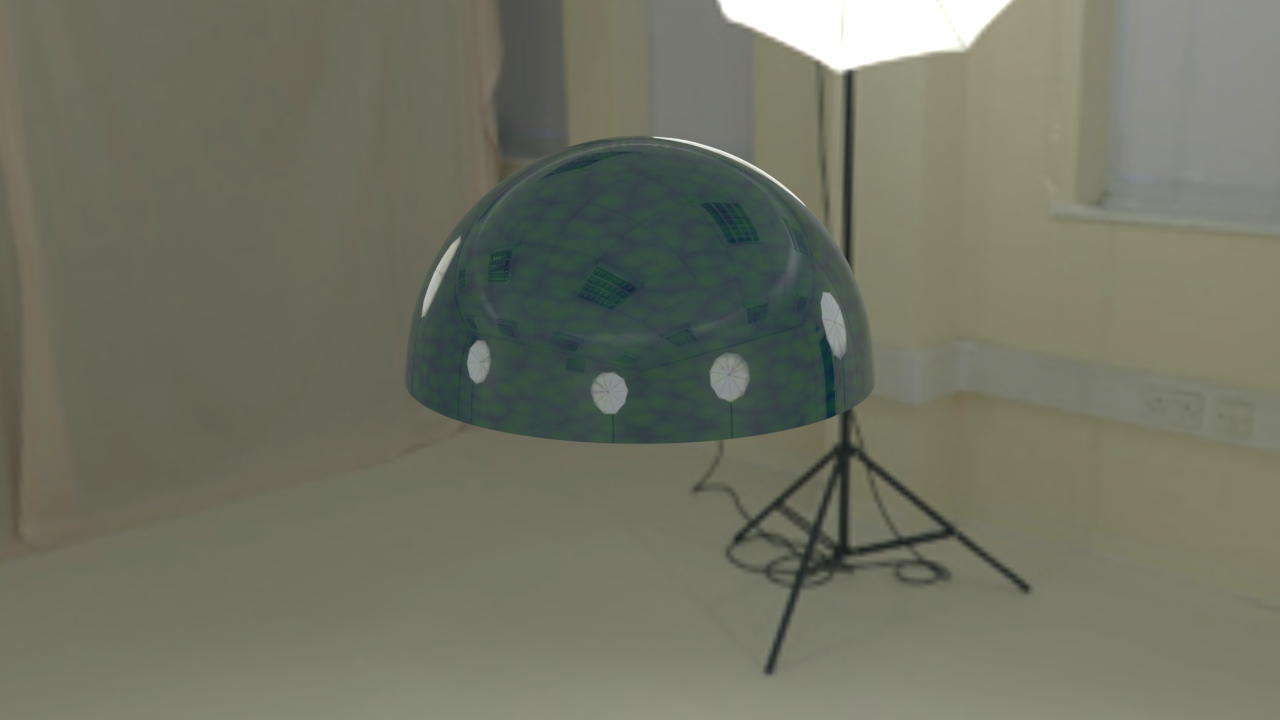
\includegraphics[width=0.33\textwidth]{mapping/mvs_alb_spec/alb_spec_0202}&
% 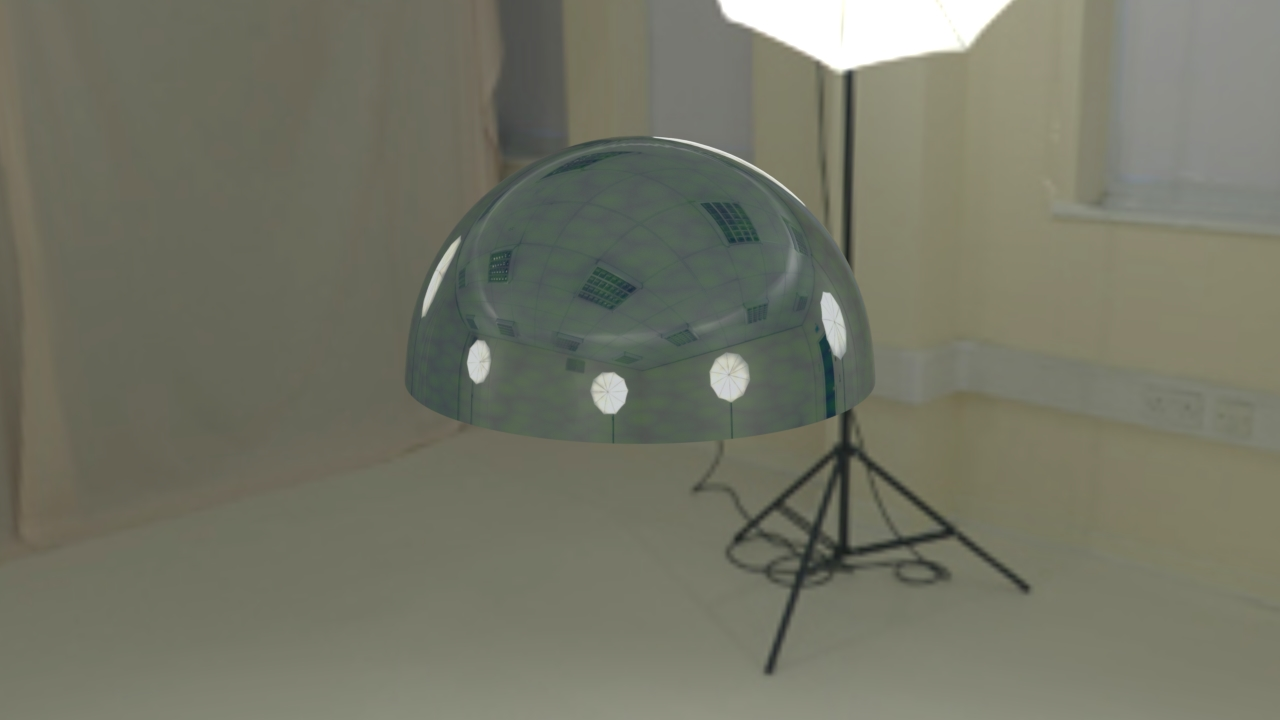
\includegraphics[width=0.33\textwidth]{mapping/mvs_alb_spec/alb_spec_0205}&
% 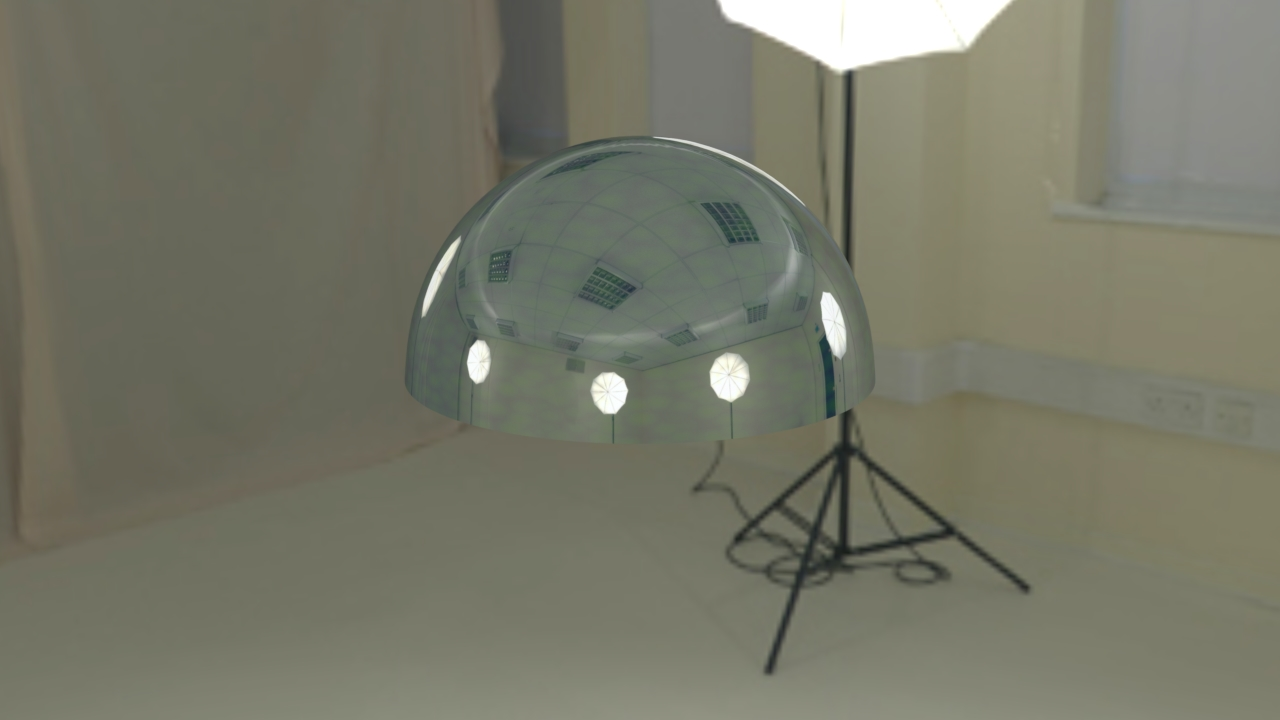
\includegraphics[width=0.33\textwidth]{mapping/mvs_alb_spec/alb_spec_0208}\\
% (a) spec: 0.2 & (b) spec: 0.5 & (c) spec: 0.8\\
% 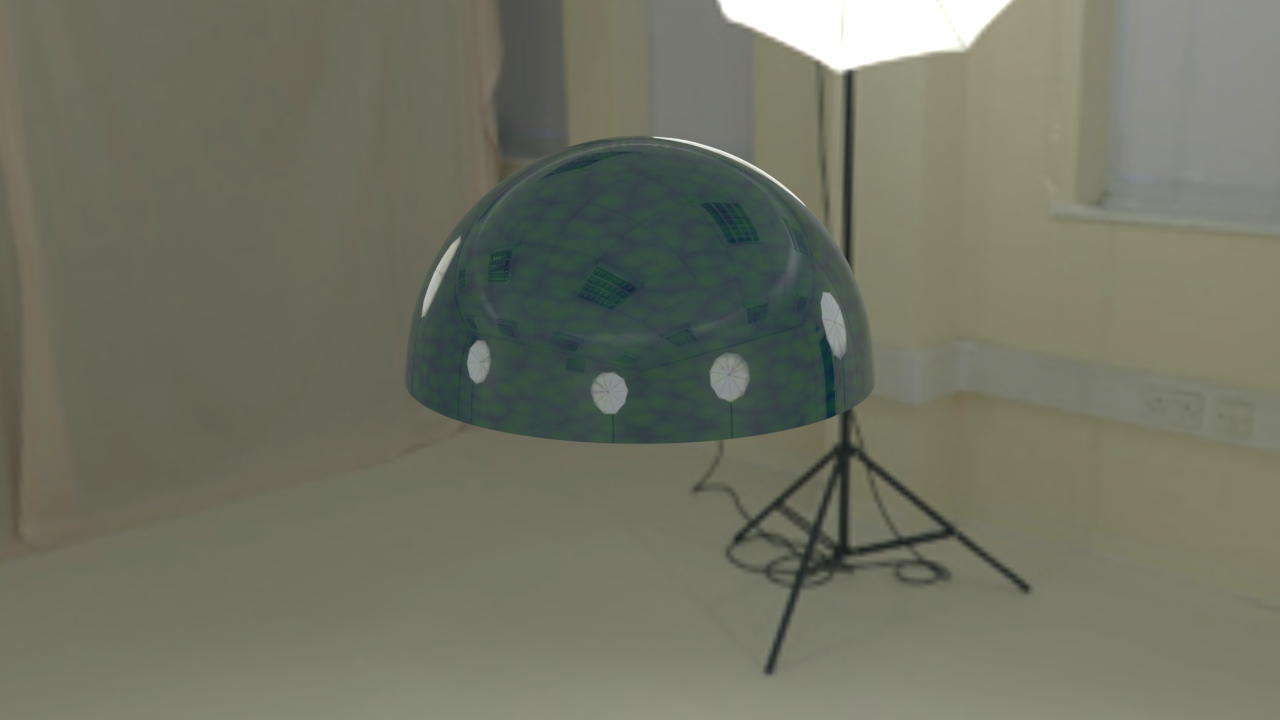
\includegraphics[width=0.33\textwidth]{mapping/mvs_alb_spec/alb_spec_0202}&
% 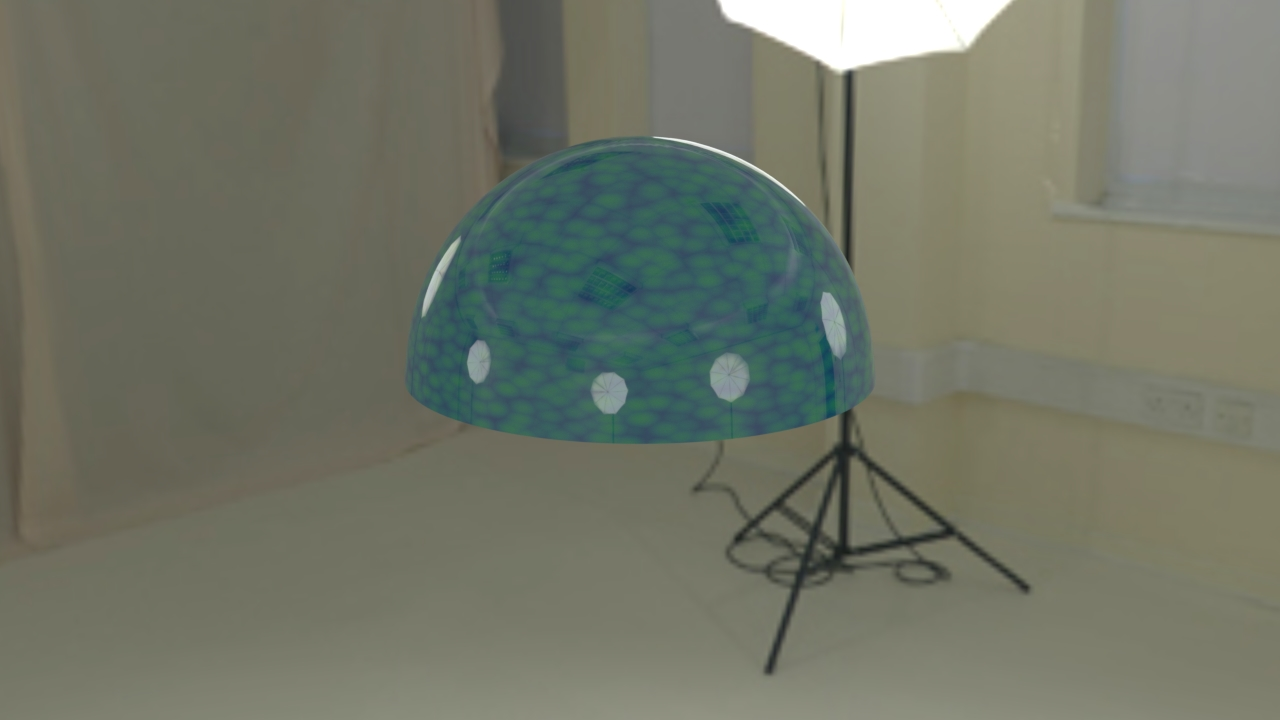
\includegraphics[width=0.33\textwidth]{mapping/mvs_alb_spec/alb_spec_0502}&
% 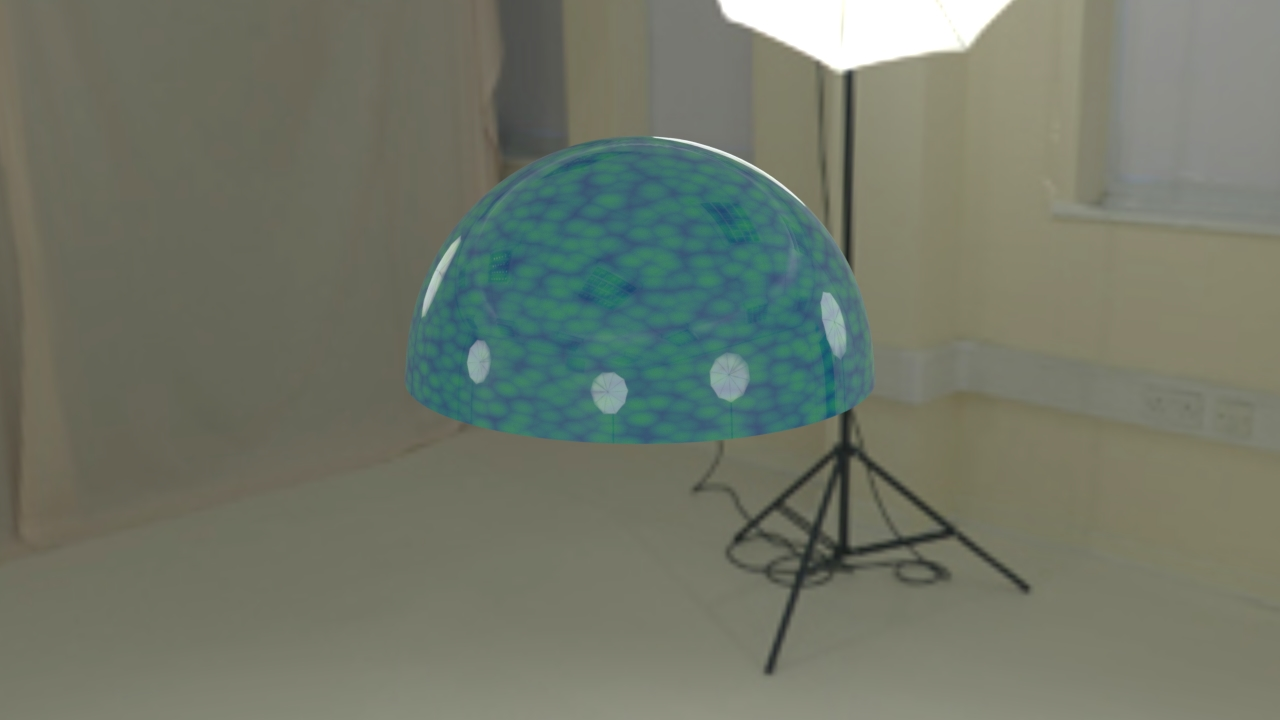
\includegraphics[width=0.33\textwidth]{mapping/mvs_alb_spec/alb_spec_0802}\\
% (d) alb: 0.2 & (e) alb: 0.5 & (f) alb: 0.8\\
% \end{tabular}
% \caption{(a)-(c). The albedo is set as 0.2, (d)-(f). The specularity is set as 0.2. According to energy conservation, as the specular component increases, the diffuse component decreases.}
% \label{fig:mvs_alb_spec}
% \end{figure}

\textbf{(e) Albedo and Roughness}
The main effects of albedo and roughness on accuracy and completeness are not significant. There is no interaction effect between albedo and roughness either.

\textbf{(f) Specularity and Roughness} 
The main effects of specular and roughness on accuracy and completeness are not significant. There is no interaction effect between spcularity and roughness either.

% surface roughness can effectively diminish the specular component and make the surface appear more diffuse. Thus, in theory, roughness should have a positive impact on the reconstruction. However, since specularity is only effective on surface with medium level texture, see Figure~\ref{fig:mvs_pairwise} (b), then roughness is only effective in this case as well. Further, since higher specular, high roughness surfaces visually resemble lower specular surfaces, and achieve similar reconstruction results as well, it makes sense to incorporate the effect of roughness to specularity, and omit roughness for simplicity.

\subsubsection{Summary: PMVS} 
Figure~\ref{fig:mvs_pairwise} demonstrates the main effect of texture, albedo and specularity on accuracy and completeness, and interaction effect between texture and specularity, albedo and specularity.

% The effective properties of PMVS are: texture, albedo, and specular, as shown in Table~\ref{tab:mvs_depend_prop}. Interestingly, we discovered that specularity has a more substantially negative impact on less textured, lower albedo surfaces. For instance, high specularity does not have a severely negative impact on highly textured surfaces.

\subsection{Main effects and interactions: EPS}
\label{sec:ps_epd}
We interpret the main effects and interactions of properties on the performance of EPS in terms of mean and standard deviation (SD) of angular error. The settings of properties are summarized in Table~\ref{tab:pairwise_prob_cond}. The performance of the algorithm in terms of two changing properties are visualized in Figure~\ref{fig:ps_pairwise}.
\begin{figure}[!htbp]
\begin{tabular}{cc}
\includegraphics[width=0.45\textwidth]{mapping/pairwise/ps_tex_alb}&
\includegraphics[width=0.45\textwidth]{mapping/pairwise/ps_tex_spec}\\
(a) & (b)\\
\includegraphics[width=0.45\textwidth]{mapping/pairwise/ps_tex_rough}&
\includegraphics[width=0.45\textwidth]{mapping/pairwise/ps_alb_spec}\\
(c) & (d)\\
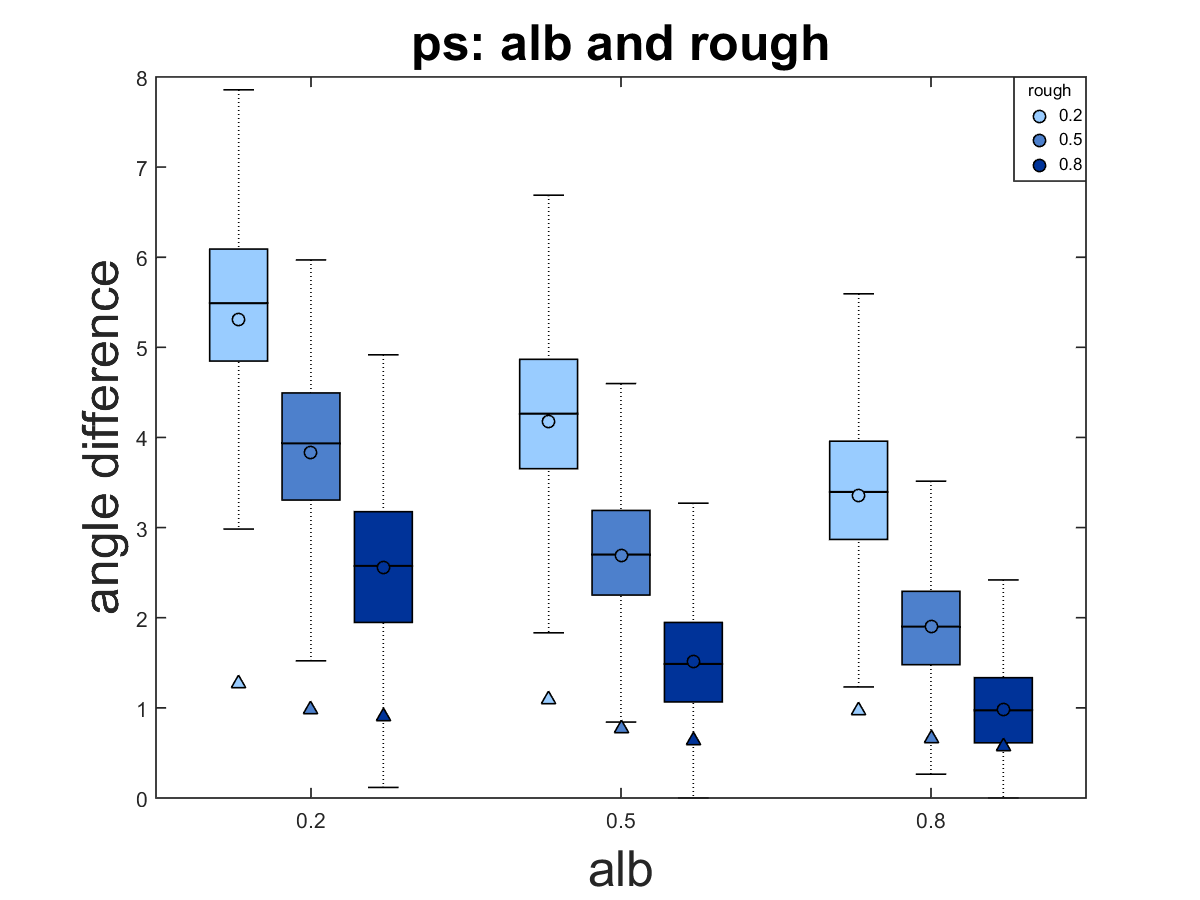
\includegraphics[width=0.45\textwidth]{mapping/pairwise/ps_alb_rough}&
\includegraphics[width=0.45\textwidth]{mapping/pairwise/ps_spec_rough}\\
(e) & (f)\\
\end{tabular}
\caption{Performance of Example-based PS under six pairwise conditions. For instance, (a) shows the performance under changing \textit{texture} and \textit{albedo} values. The property values are assigned based on the settings in Table~\ref{tab:pairwise_prob_cond} (a).}
\label{fig:ps_pairwise}
\end{figure}

\textbf{(a) Texture and Albedo} 
The main effects of texture on mean and SD of angular error, and the main effect of albedo on SD of angular error are not significant. The main effect of albedo on mean value of angular error is significant such that the angular error decreases as the albedo increases. There is no significant interaction effect between texture and albedo.

\textbf{(b) Texture and Specularity} 
The main effects of texture on mean and SD of angular error are not significant whereas the main effects of speculairty are significant such that both values increases as specularity increases. There is no significant interaction effect between texture and specularity in terms of mean and SD of angular error.
% \begin{figure}[!htbp]
% \centering
% \begin{tabular}{c|ccc}
% Image & Normal map & Height map & Angular error\\
% \hline\\
% \includegraphics[width=0.33\textwidth]{mapping/ps_tex_spec/0502_0001}&
% 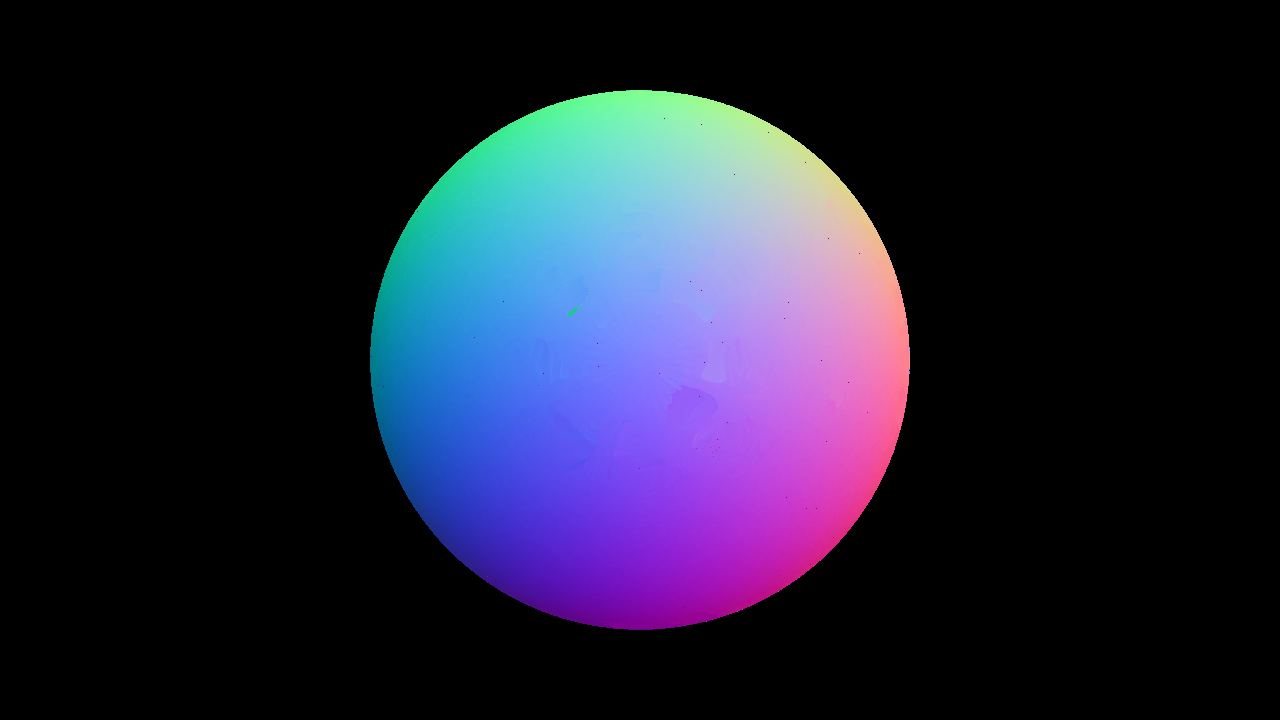
\includegraphics[width=0.33\textwidth]{mapping/ps_tex_spec/0502_normal}&
% 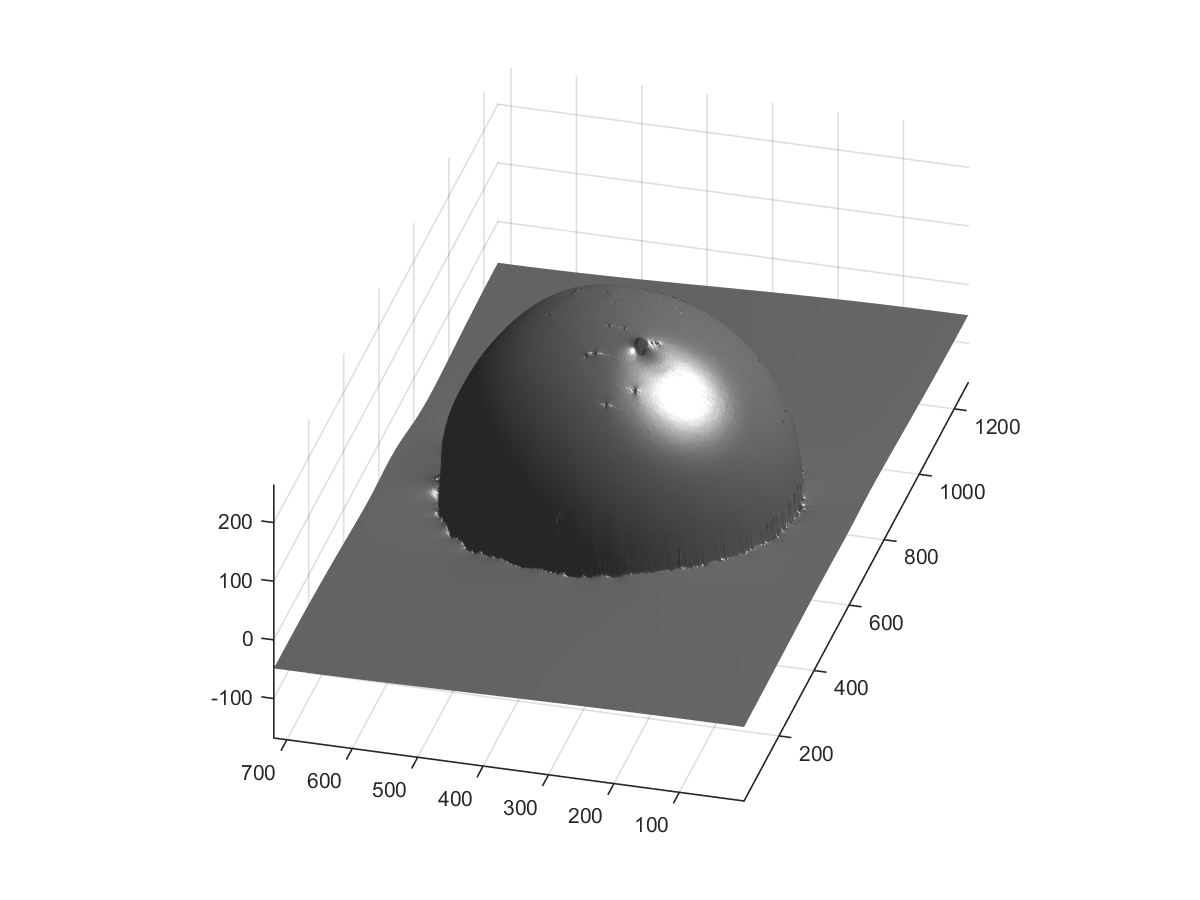
\includegraphics[width=0.25\textwidth]{mapping/ps_tex_spec/0502_dmap}&
% \includegraphics[width=0.06\textwidth]{mapping/ps_tex_spec/0502_ang_error}\\
%  & spec: 0.2 & \\
% 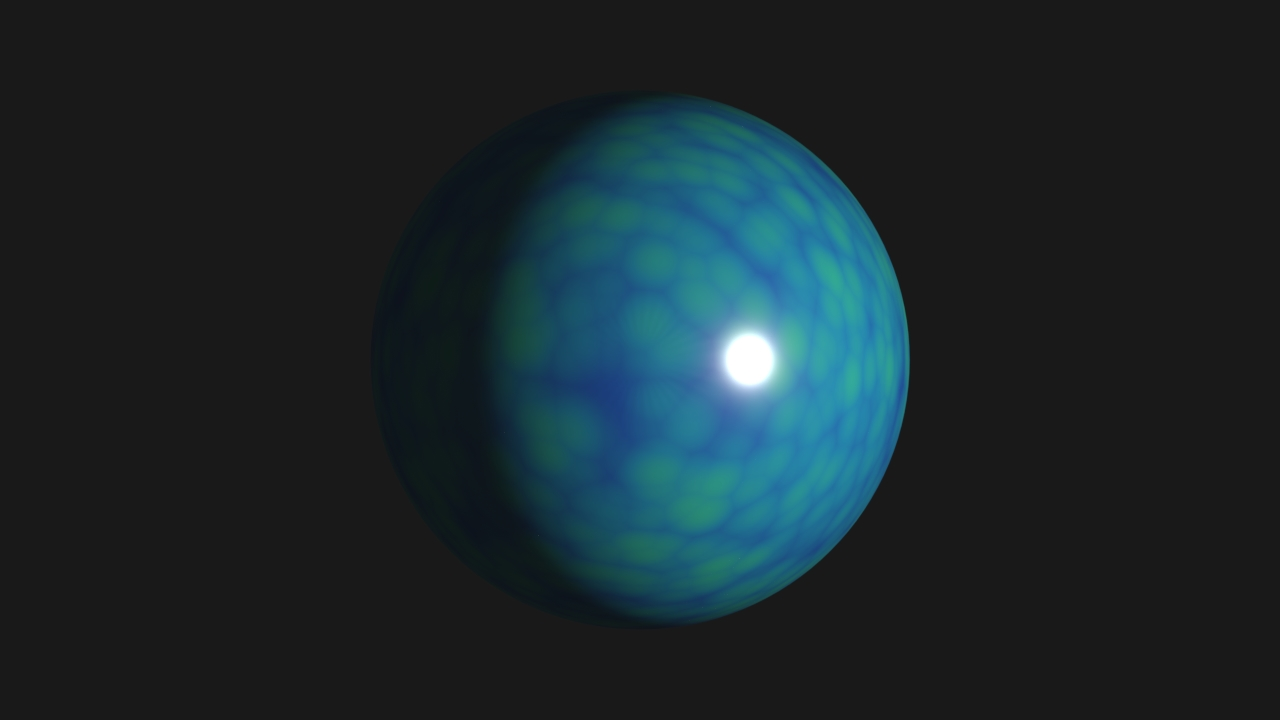
\includegraphics[width=0.33\textwidth]{mapping/ps_tex_spec/0505_0001}&
% 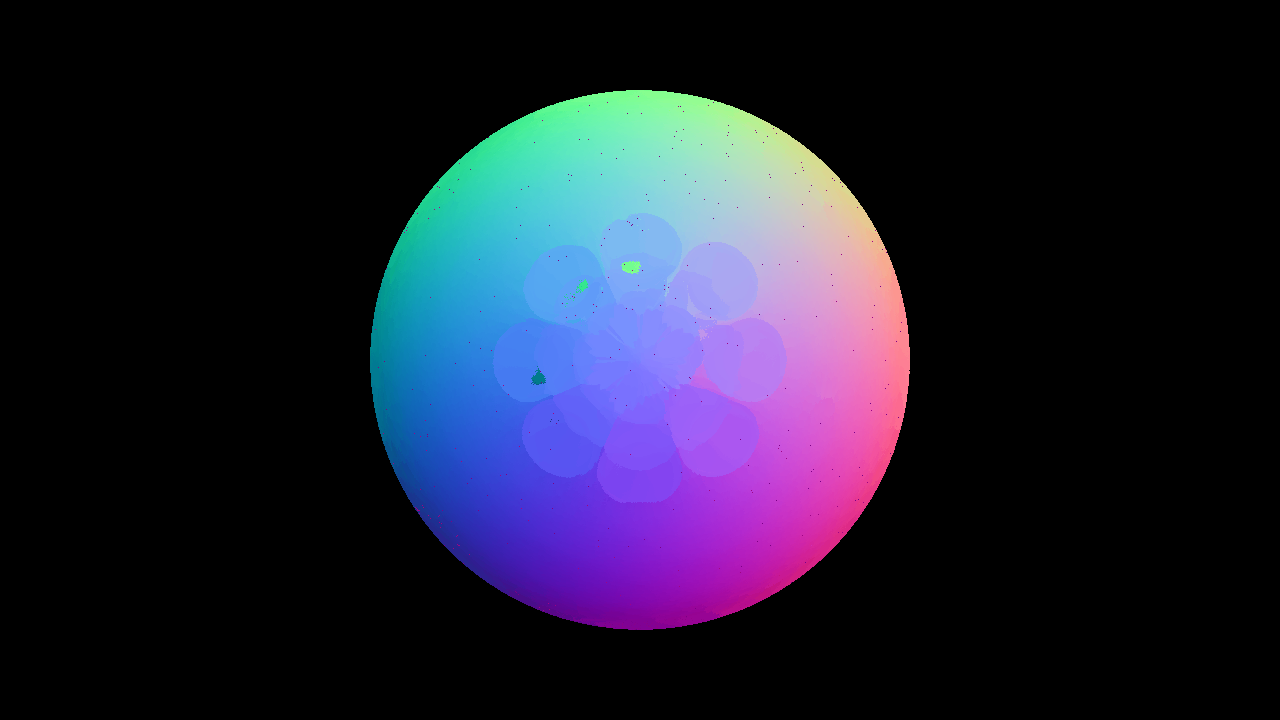
\includegraphics[width=0.33\textwidth]{mapping/ps_tex_spec/0505_normal}&
% 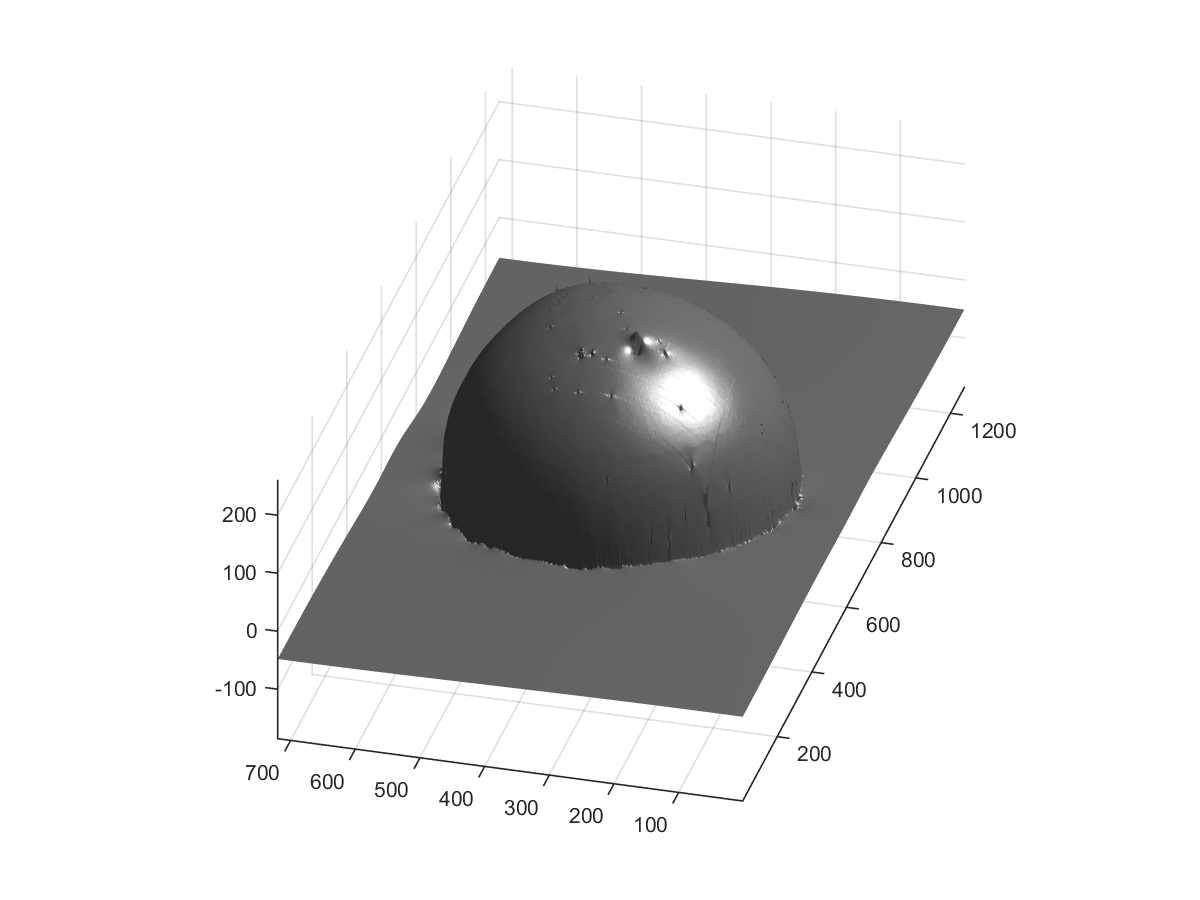
\includegraphics[width=0.25\textwidth]{mapping/ps_tex_spec/0505_dmap}&
% \includegraphics[width=0.06\textwidth]{mapping/ps_tex_spec/0505_ang_error}\\
%  & spec: 0.5 & \\
% 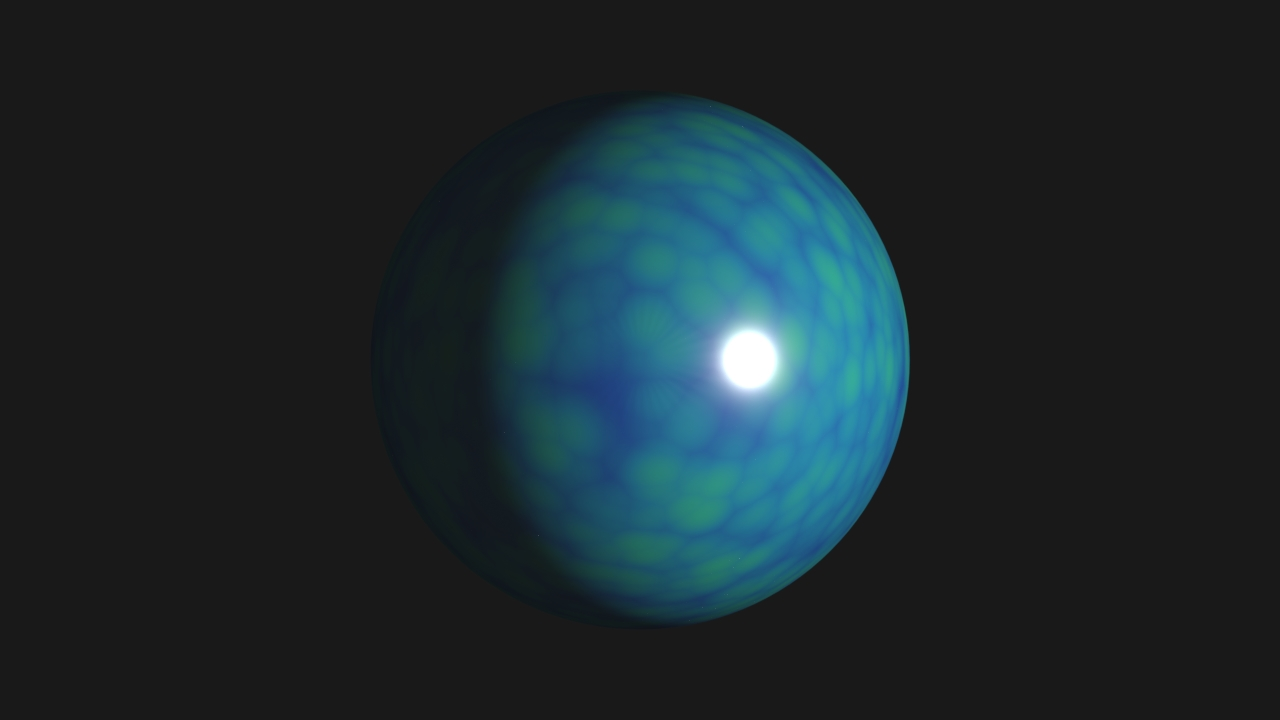
\includegraphics[width=0.33\textwidth]{mapping/ps_tex_spec/0508_0001}&
% 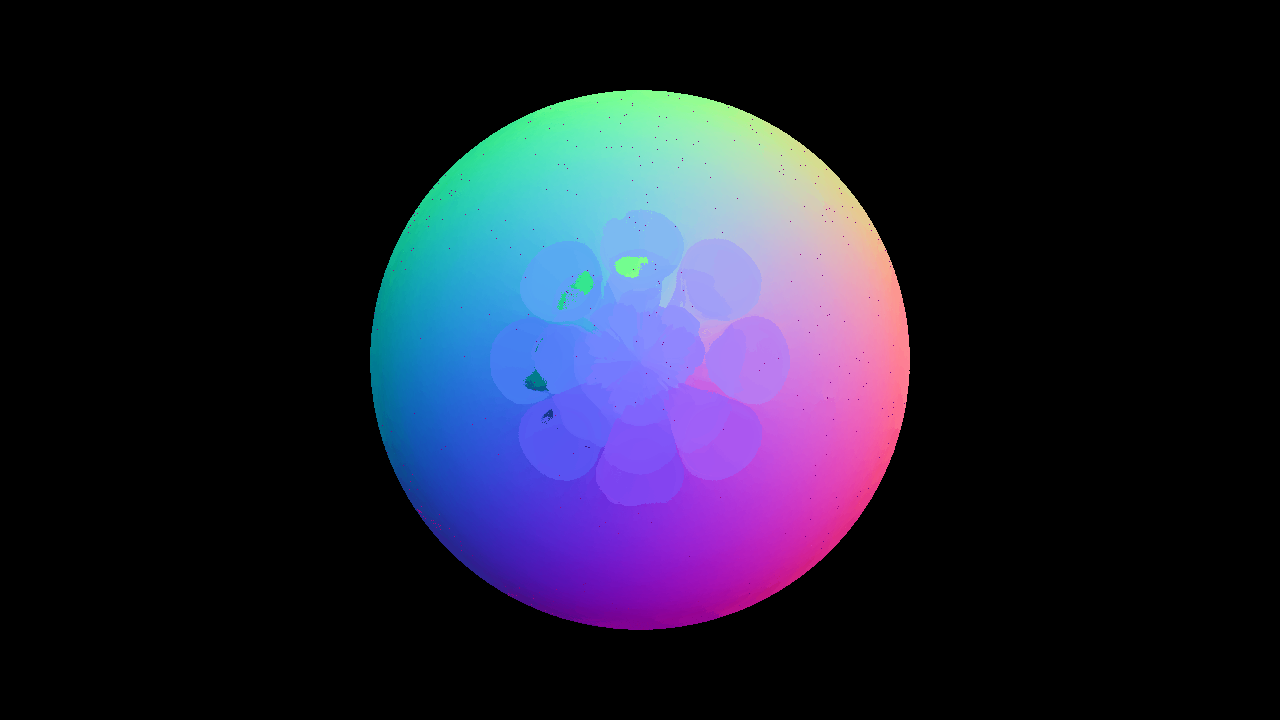
\includegraphics[width=0.33\textwidth]{mapping/ps_tex_spec/0508_normal}&
% 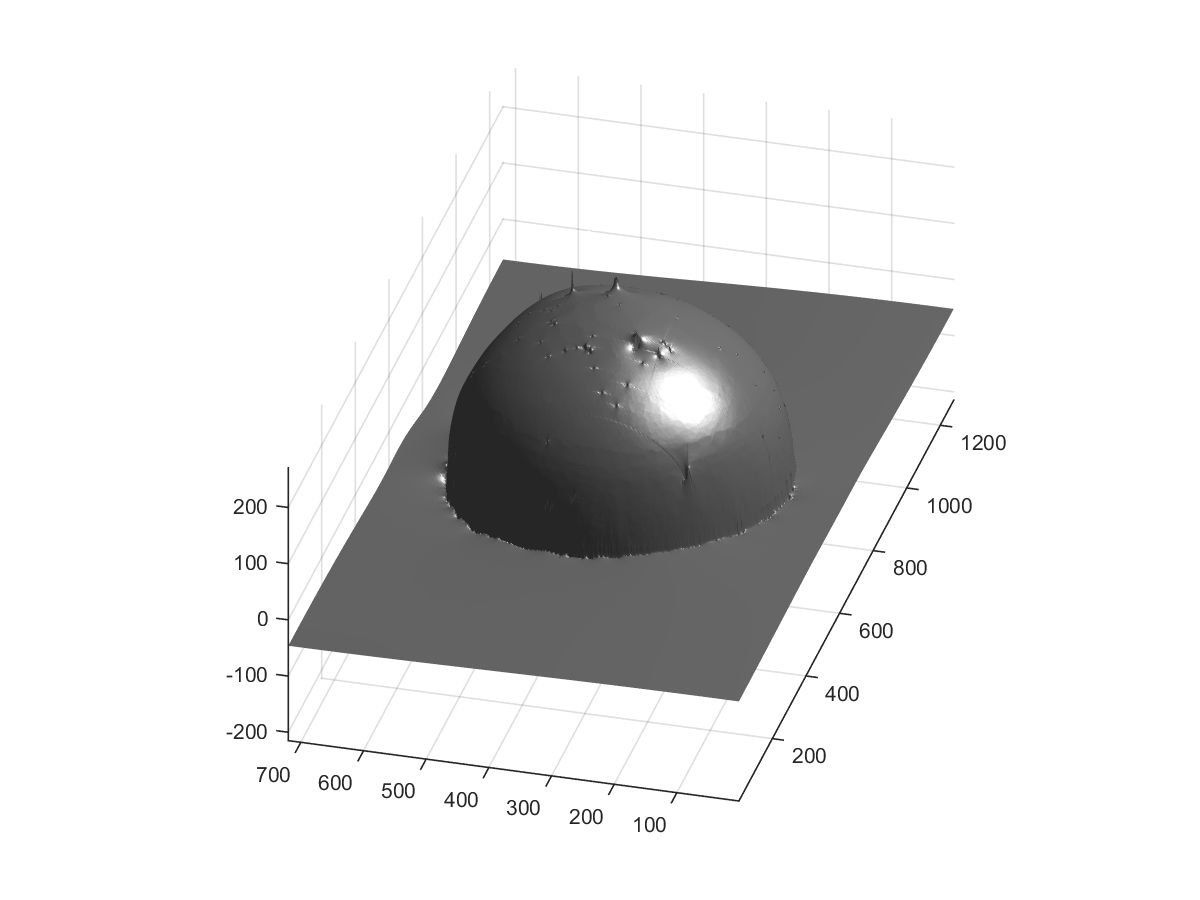
\includegraphics[width=0.25\textwidth]{mapping/ps_tex_spec/0508_dmap}&
% \includegraphics[width=0.06\textwidth]{mapping/ps_tex_spec/0508_ang_error}\\
%  & spec: 0.8 & \\
% \end{tabular}
% \caption{(a)-(c). The texture is set as 0.5. The estimated normal map and recovered surface becomes consistently worse as the specular level rises, which is consistent with the quantitative results from Figure~\ref{fig:ps_pairwise} (b).}
% \label{fig:ps_tex_spec}
% \end{figure}

\textbf{(c) Texture and Roughness} 
The main effects of texture on mean and SD of angular error, and the main effect of roughness on SD of angular error are not significant whereas the main effect of roughness on mean of angular error is significant such that the mean angular error decreases as roughness increases. There is no interaction between texture and roughness in terms of mean and SD of angular error.

\textbf{(d) Albedo and Specular} 
The main effects of albedo and specularity on mean and SD of angular error are significant such that the mean and angular error decreases as albedo increases or specularity decreases. There is no significant interaction effect between albedo and specularity as the colour changes monotonically along the diagonal.
% the albedo has a positive impact on normal estimation (see Figure~\ref{fig:ps_alb_spec} (a)-(c)), whereas the specularity has a negative impact on normal estimation (see Figure~\ref{fig:ps_alb_spec} (d)-(f)).
% \begin{figure}[!htbp]
% \centering
% \begin{tabular}{c|ccc}
% Image & Normal map & Height map & Angular error\\
% \hline\\
% % 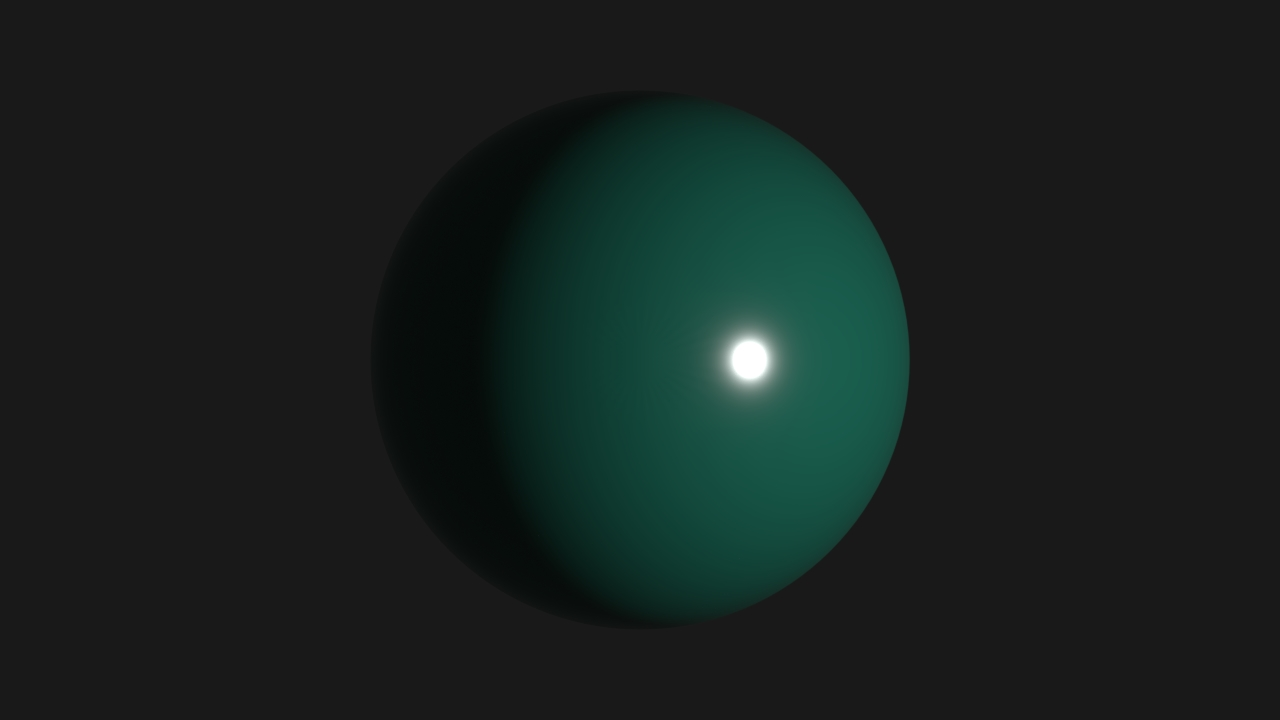
\includegraphics[width=0.33\textwidth]{mapping/ps_alb_spec/0202_0001}&
% % 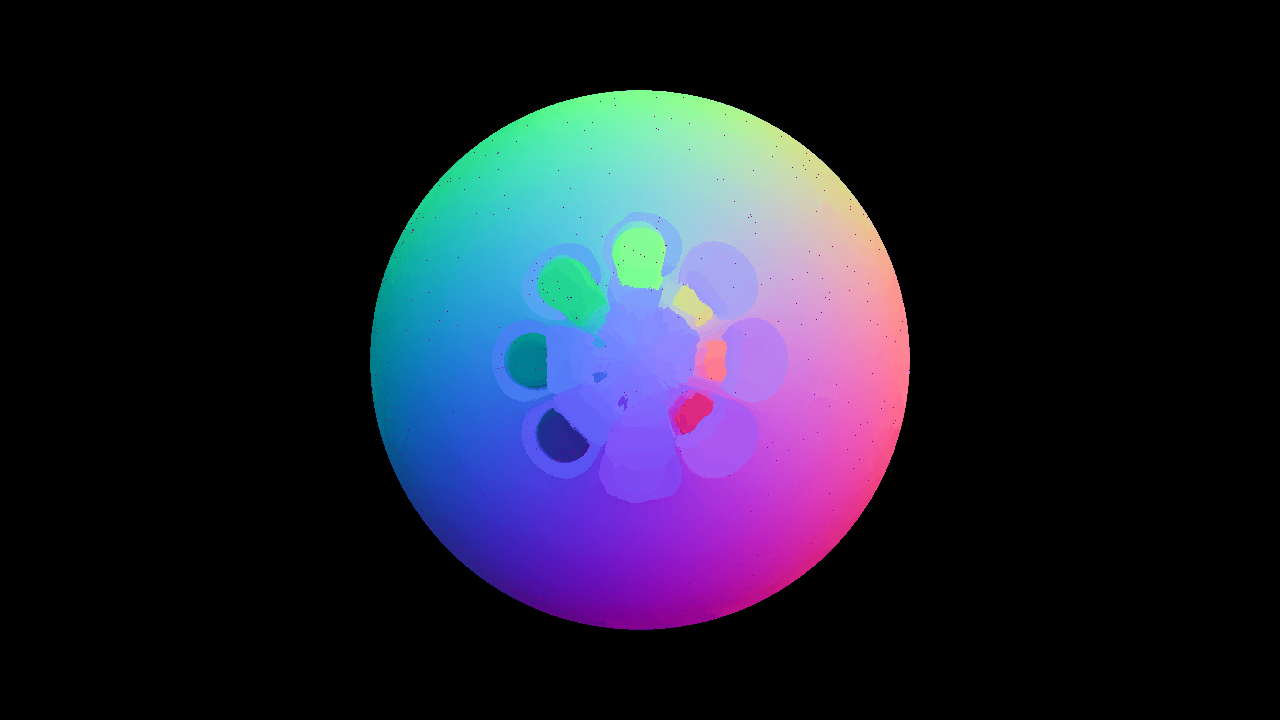
\includegraphics[width=0.33\textwidth]{mapping/ps_alb_spec/0202_normal}&
% % 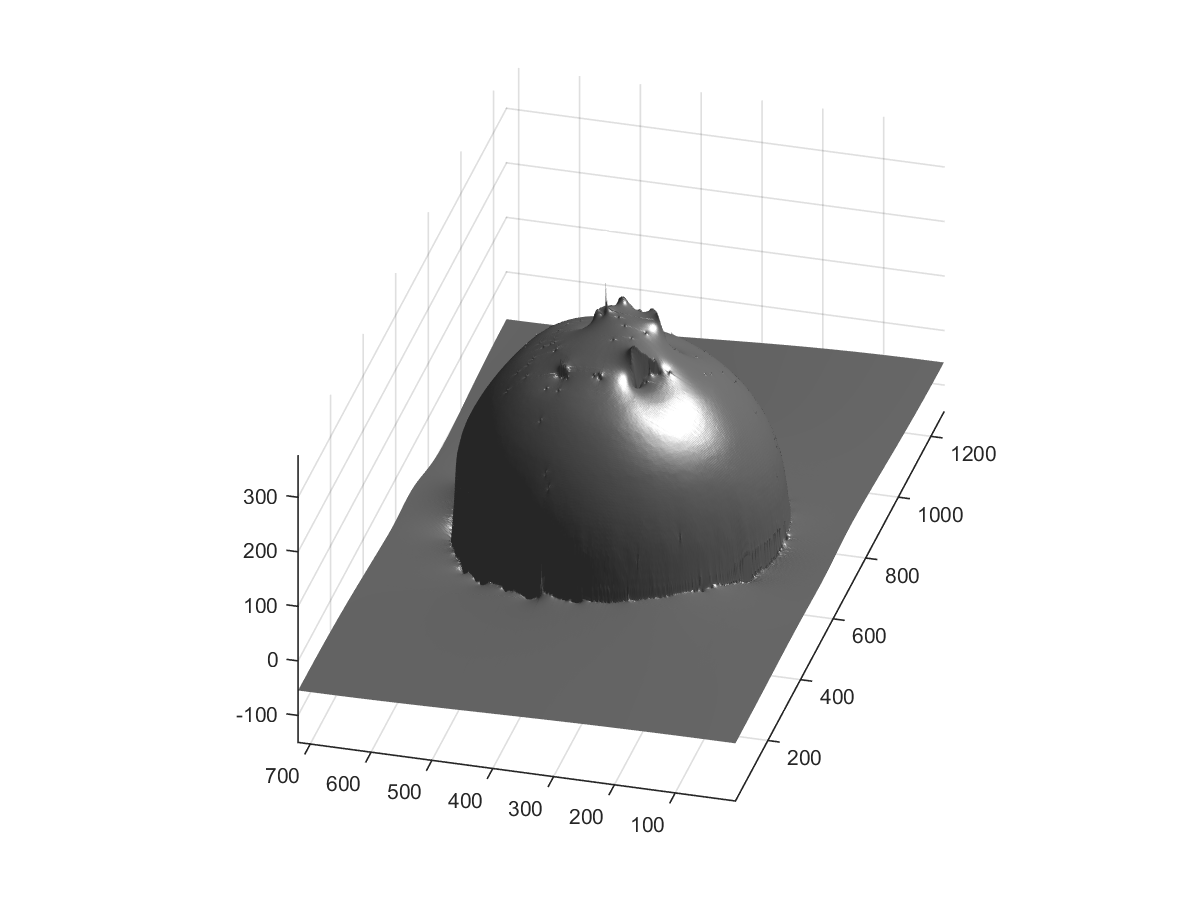
\includegraphics[width=0.25\textwidth]{mapping/ps_alb_spec/0202_dmap}&
% % \includegraphics[width=0.06\textwidth]{mapping/ps_alb_spec/0202_ang_error}\\
% %  & (a) albedo: 0.2, spec: 0.2 & \\
% 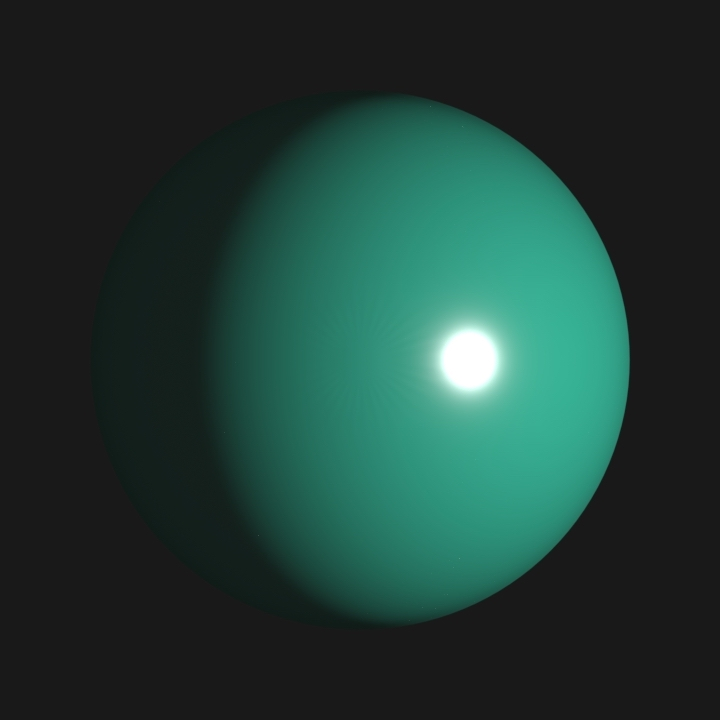
\includegraphics[width=0.33\textwidth]{mapping/ps_alb_spec/0802_0001}&
% 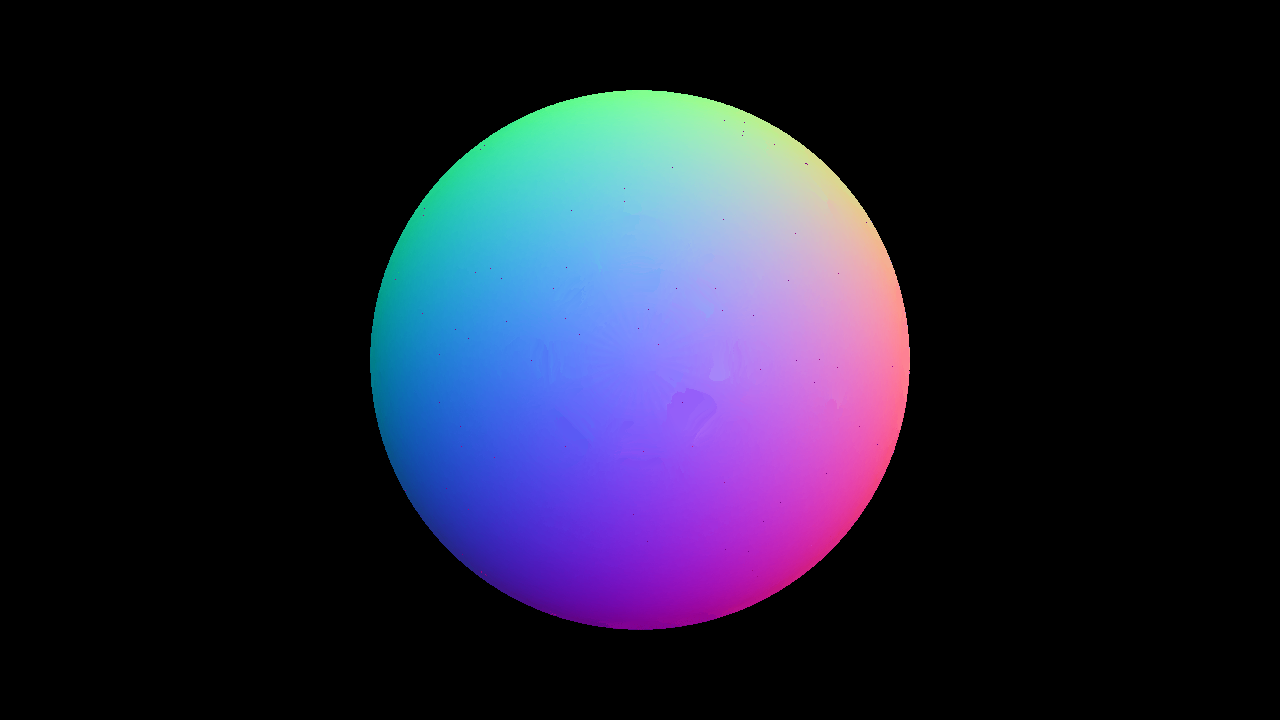
\includegraphics[width=0.33\textwidth]{mapping/ps_alb_spec/0802_normal}&
% 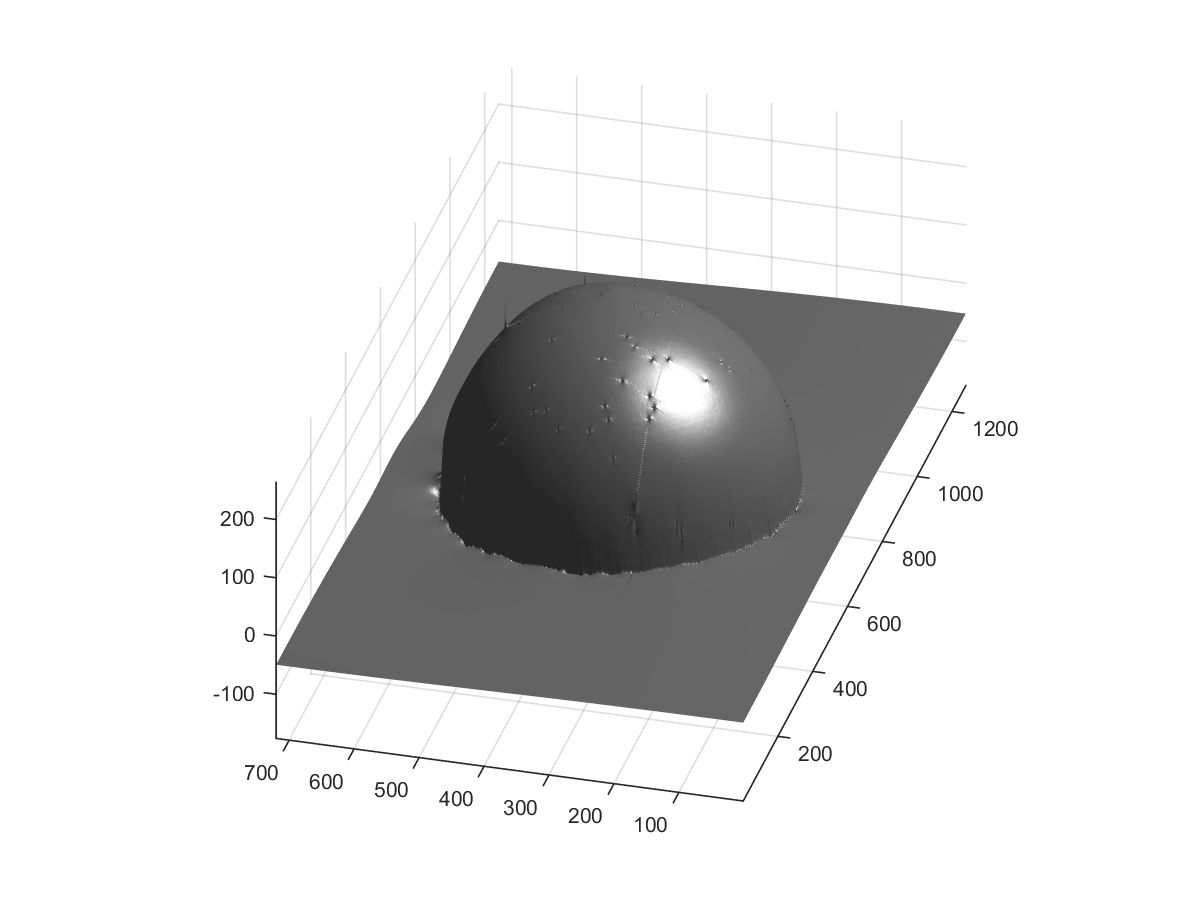
\includegraphics[width=0.25\textwidth]{mapping/ps_alb_spec/0802_dmap}&
% \includegraphics[width=0.06\textwidth]{mapping/ps_alb_spec/0802_ang_error}\\
%  & (a) albedo: 0.8, spec: 0.2 & \\
% \includegraphics[width=0.33\textwidth]{mapping/ps_alb_spec/0502_0001}&
% \includegraphics[width=0.33\textwidth]{mapping/ps_alb_spec/0502_normal}&
% \includegraphics[width=0.25\textwidth]{mapping/ps_alb_spec/0502_dmap}&
% \includegraphics[width=0.06\textwidth]{mapping/ps_alb_spec/0502_ang_error}\\
%  & (b) albedo: 0.5, spec: 0.2 & \\
% \includegraphics[width=0.33\textwidth]{mapping/ps_alb_spec/0202_0001}&
% \includegraphics[width=0.33\textwidth]{mapping/ps_alb_spec/0202_normal}&
% \includegraphics[width=0.25\textwidth]{mapping/ps_alb_spec/0202_dmap}&
% \includegraphics[width=0.06\textwidth]{mapping/ps_alb_spec/0202_ang_error}\\
%  & (c) albedo: 0.2, spec: 0.2 & \\
% \includegraphics[width=0.33\textwidth]{mapping/ps_alb_spec/0205_0001}&
% \includegraphics[width=0.33\textwidth]{mapping/ps_alb_spec/0205_normal}&
% \includegraphics[width=0.25\textwidth]{mapping/ps_alb_spec/0205_dmap}&
% \includegraphics[width=0.06\textwidth]{mapping/ps_alb_spec/0205_ang_error}\\
%  & (d) albedo: 0.2, spec: 0.5 & \\
% \includegraphics[width=0.33\textwidth]{mapping/ps_alb_spec/0208_0001}&
% \includegraphics[width=0.33\textwidth]{mapping/ps_alb_spec/0208_normal}&
% \includegraphics[width=0.25\textwidth]{mapping/ps_alb_spec/0208_dmap}&
% \includegraphics[width=0.06\textwidth]{mapping/ps_alb_spec/0208_ang_error}\\
%  & (e) albedo: 0.2, spec: 0.8 & \\
% \end{tabular}
% \caption{According to energy conservation, as the specular component increases, the diffuse component decreases. (a)-(c): the estimated normal map and recovered height map become consistently worse as the albedo decreases; (c)-(e): the estimated normal map and recovered height map become consistently worse as the specularity increases.}
% \label{fig:ps_alb_spec}
% \end{figure}

\textbf{(e) Albedo and Roughness} 
The main effects of albedo and roughness on SD of angular error are not significant whereas the main effects on mean of angular error is significant such that the mean angular error increases as the albedo or roughness increases. There is no interaction effect between albedo and roughness.

\textbf{(f) Specular and Roughness} 
The main effect of specularity on mean and SD of angular error is significant such that the value increases as the specularity increases. There is an interaction effect between specularity and roughness. More specifically, the mean and SD of angular error get worse for medium roughness, which is counter-intuitive at first sight. However, we argue that it's because the roughness is not strong enough to counteract the specular component, causing a smoothed and blurred specular region with larger area, thus leading to a poorer normal estimation. See Figure~\ref{fig:ps_spec_rough} for visual examples.
\begin{figure}[!htbp]
\centering
\begin{tabular}{cccc}
  Image & Normal map & Height map & Angular error\\
  \hline\\
  \includegraphics[width=0.2\textwidth]{mapping/ps_spec_rough/0802_0001}&
  \includegraphics[width=0.2\textwidth]{mapping/ps_spec_rough/0802_normal}&
  \includegraphics[width=0.2\textwidth]{mapping/ps_spec_rough/0802_dmap}&
  \includegraphics[width=0.07\textwidth]{mapping/ps_spec_rough/0802_ang_error}\\
  \multicolumn{4}{c}{(a). roughness: 0.2}\\
  \includegraphics[width=0.2\textwidth]{mapping/ps_spec_rough/0805_0001}&
  \includegraphics[width=0.2\textwidth]{mapping/ps_spec_rough/0805_normal}&
  \includegraphics[width=0.2\textwidth]{mapping/ps_spec_rough/0805_dmap}&
  \includegraphics[width=0.07\textwidth]{mapping/ps_spec_rough/0805_ang_error}\\
  \multicolumn{4}{c}{(b). roughness: 0.5}\\
  \includegraphics[width=0.2\textwidth]{mapping/ps_spec_rough/0808_0001}&
  \includegraphics[width=0.2\textwidth]{mapping/ps_spec_rough/0808_normal}&
  \includegraphics[width=0.2\textwidth]{mapping/ps_spec_rough/0808_dmap}&
  \includegraphics[width=0.07\textwidth]{mapping/ps_spec_rough/0808_ang_error}\\
  \multicolumn{4}{c}{(c). roughness: 0.8}\\
\end{tabular}
\caption{The effect of roughness on PS. Albedo is set as 0.8, and specular is set as 0.8. The first column shows the input images, the second column shows the estimated normal map, the third column shows the integrated surface, and last column shows the angular error. We can see from the qualitative results (normal map and height map), and quantitative result (angular error) that a medium level roughness would lead to worse normal estimation since it blurs the specular lobe.}
\label{fig:ps_spec_rough}
\end{figure}

\subsubsection{Summary: EPS} 
Figure~\ref{fig:ps_pairwise} demonstrate the main effect of albedo, specularity ,and roughness on angular error, and interaction effect between specularity and roughness.

% The properties that have an impact on EPS are: albedo, specularity, and roughness, as shown in Table~\ref{tab:ps_depend_prop}. Interestingly, we have discovered that medium level roughness can have a negative impact on normal estimation by blur the specular lobe, as shown in Figure~\ref{fig:ps_spec_rough}.
% \begin{table}[!htbp]
%   \centering
%   \begin{tabular}{l*{5}{c}}
%   \hline
%   \textbf{Metric} & Texture & Albedo & Specular & Roughness\\
%   \hline
%   Angle difference & \ding{55} & \checkmark & \checkmark & \checkmark\\
%   \hline
%   \end{tabular}
%   \caption{The \textit{effective problem domain} of EPS in terms of the \textit{angular error}.}
%   \label{tab:ps_depend_prop}
% \end{table}

\subsection{Main effects and interactions: GSL}
\label{sec:sl_epd}
We interpret the main effects and interactions of properties on the performance of PMVS in terms of accuracy and completeness. The settings of properties are summarized in Table~\ref{tab:pairwise_prob_cond}. The performance of the algorithm in terms of two changing properties are visualized in Figure~\ref{fig:sl_pairwise}.
\begin{figure}[!htbp]
\begin{tabular}{cc}
\includegraphics[width=0.45\textwidth]{mapping/pairwise/sl_tex_alb}&
\includegraphics[width=0.45\textwidth]{mapping/pairwise/sl_tex_spec}\\
(a) & (b) \\
\includegraphics[width=0.45\textwidth]{mapping/pairwise/sl_tex_rough}&
\includegraphics[width=0.45\textwidth]{mapping/pairwise/sl_alb_spec}\\
(c) & (d) \\
\includegraphics[width=0.45\textwidth]{mapping/pairwise/sl_alb_rough}&
\includegraphics[width=0.45\textwidth]{mapping/pairwise/sl_spec_rough}\\
(e) & (f)\\
\end{tabular}
\caption{Performance of Gray-encoded SL under six pairwise conditions. For instance, (a) shows the performance under changing \textit{texture} and \textit{albedo} values. The property values are assigned based on settings in Table~\ref{tab:pairwise_prob_cond} (a).}
\label{fig:sl_pairwise}
\end{figure}

\textbf{(a) Texture and Albedo} 
The main effect of texture on accuracy and completeness and the main effect of albedo on accuracy is not significant. The main effect of albedo on completeness is significant such that the results increases as the albedo increases. There is no significant interaction effect between texture and albedo.

\textbf{(b) Texture and Specularity} 
The main effect of texture on accuracy and completeness and the main effect of specularity on accuracy is not significant. The main effect of specularity on completeness is significant such that the results decreases as the specularity increases. There is no significant interaction effect between texture and specularity.

\textbf{(c) Texture and Roughness} 
The main effect of texture on accuracy and completeness and the main effect of roughness on accuracy is not significant. The main effect of roughness on completeness is significant such that the results increases as the roughness increases. There is no significant interaction effect between texture and roughness.

\textbf{(d) Albedo and Specularity} 
The main effects of albedo and specularity on accuracy are not significant whereas the main effects on completeness are significant such that the results increase as albedo increase or specularity decreases. There is no significant interaction effect between albedo and specularity.

% albedo has a positive effect (see Figure~\ref{fig:sl_alb_spec} (a)-(c)) whereas specularity has a negative effect on completeness (see Figure~\ref{fig:sl_alb_spec} (d)-(f)). Interestingly, similar to EPS, the positive effect of albedo gets more significant with higher specularity while the negative effect of specularity becomes less substantial as albedo increases (see Figure~\ref{fig:sl_pairwise} (d)). Neither property has a significant effect on accuracy.
% \begin{figure}[!htbp]
% \centering
% \begin{tabular}{ccc}
% \includegraphics[width=0.33\textwidth]{mapping/sl_alb_spec/sl_00020202}&
% \includegraphics[width=0.33\textwidth]{mapping/sl_alb_spec/sl_00050202}&
% \includegraphics[width=0.33\textwidth]{mapping/sl_alb_spec/sl_00080202}\\
% (a) albedo: 0.2 & (b) albedo: 0.5 & (c) albedo: 0.8\\
% \includegraphics[width=0.33\textwidth]{mapping/sl_alb_spec/sl_00020202}&
% \includegraphics[width=0.33\textwidth]{mapping/sl_alb_spec/sl_00020502}&
% \includegraphics[width=0.33\textwidth]{mapping/sl_alb_spec/sl_00020802}\\
% (d) specular: 0.2 & (e) specular: 0.5 & (f) specular: 0.8\\
% \end{tabular}
% \caption{(a)-(c): the specular is set as 0.2, albedo has a positive effect on completeness; (d)-(e): the albedo is set as 0.2, specular has a negative effect on completeness.}
% \label{fig:sl_alb_spec}
% \end{figure}

\textbf{(e) Albedo and Roughness} 
The main effects of albedo and roughness on accuracy, and the main effect of roughness on completeness are not significant. The main effect of albedo on completeness is significant such that the results increases as the albedo increases. There is no significant interaction effect between albedo and roughness.

\textbf{(f) Specular and Roughness} 
The main effects of specularity and roughness on accuracy. The main effect of roughness and specularity on completeness is significant such that the results increases as the roughness increases or specularity decreases. There is no significant interaction effect between specularity and roughness.
% specular has a negative effect (see Figure~\ref{fig:sl_spec_rough} (a)-(c)). Interestingly, the effect of roughness also resembles that of EPS, \ie medium level roughness has a negative impact on completeness (see Figure~\ref{fig:sl_spec_rough} (d)-(f)). Neither property has a significant effect on accuracy.
% \begin{figure}[!htbp]
% \centering
% \begin{tabular}{ccc}
% \includegraphics[width=0.33\textwidth]{mapping/sl_spec_rough/sl_00050202}&
% \includegraphics[width=0.33\textwidth]{mapping/sl_spec_rough/sl_00050502}&
% \includegraphics[width=0.33\textwidth]{mapping/sl_spec_rough/sl_00050802}\\
% (a) specular: 0.2 & (b) specular: 0.5 & (c) specular: 0.8\\
% \includegraphics[width=0.33\textwidth]{mapping/sl_spec_rough/sl_00050802}&
% \includegraphics[width=0.33\textwidth]{mapping/sl_spec_rough/sl_00050805}&
% \includegraphics[width=0.33\textwidth]{mapping/sl_spec_rough/sl_00050808}\\
% (d) roughness: 0.2 & (e) roughness: 0.5 & (f) roughness: 0.8\\
% \end{tabular}
% \caption{(a)-(c): the roughness is set as 0.2, and specular has a negative effect on completeness; (d)-(e): the specular is set as 0.8, roughness has a positive effect on completeness.}
% \label{fig:sl_spec_rough}
% \end{figure}

\subsubsection{Summary: GSL}
Figure~\ref{fig:sl_pairwise} demonstrates the main effect of albedo, specularity ,and roughness on angular error, and no significant interaction effect is found.
% The properties that have an effect on the GSL are: texture, albedo, specular, as shown in Table~\ref{tab:sl_depend_prop}. The albedo has a more significant impact with lower specularity, while specularity has a more substantial impact with low albedo. Roughness can cause a blurred specular region, thus leading to decreased completeness.
% \begin{table}[!htbp]
%   \centering
%   \begin{tabular}{l*{4}{c}}
%   \hline
%   \textbf{Metric} & Texture & Albedo & Specular & Roughness\\
%   \hline
%   Accuracy & \ding{55} & \ding{55} & \ding{55} & \ding{55}\\
%   Completeness & \ding{55} & \checkmark & \checkmark & \checkmark\\
%   \hline
%   \end{tabular}
%   \caption{The \textit{effective problem domain} of GSL in terms of accuracy and completeness.}
%   \label{tab:sl_depend_prop}
% \end{table}

\section{Construction of Mapping}
We evaluate the performance of algorithms under the factorial combination of properties that have main effects on performance in terms of accuracy, completeness or angular error. The performance is compared with those of baseline methods. Specifically, the accuracy, completeness, and angular error of baseline methods are subtracted from the selected algorithms. We inverse the results of accuracy so that better reconstruction have positive values. The resulting figures are shown in Figure~\ref{fig:lookup_table}. The conditions where the quantitative measures are above zeros are considered conditions where the corresonding algorithms work. The mapping is essentially a look-up table that returns a list of algorithms that can achieve successful reconstruction given a problem condition. We determine the success of reconstruction by comparing the result to that of baseline methods.

\begin{sidewaysfigure*}[!htbp]
\centering
\begin{tabular}{ccc}
\includegraphics[width=0.3\textwidth]{mapping/lookup_table/mvs_texture_02.eps} &
\includegraphics[width=0.3\textwidth]{mapping/lookup_table/mvs_texture_05.eps} &
\includegraphics[width=0.3\textwidth]{mapping/lookup_table/mvs_texture_08.eps}\\
\multicolumn{3}{c}{(a). Look-up table of PMVS.}\\
\includegraphics[width=0.3\textwidth]{mapping/lookup_table/ps_albedo_02.eps} &
\includegraphics[width=0.3\textwidth]{mapping/lookup_table/ps_albedo_05.eps} &
\includegraphics[width=0.3\textwidth]{mapping/lookup_table/ps_albedo_08.eps}\\
\multicolumn{3}{c}{(b). Look-up table of EPS.}\\
\includegraphics[width=0.3\textwidth]{mapping/lookup_table/sl_albedo_02.eps} &
\includegraphics[width=0.3\textwidth]{mapping/lookup_table/sl_albedo_05.eps} &
\includegraphics[width=0.3\textwidth]{mapping/lookup_table/sl_albedo_08.eps}\\
\multicolumn{3}{c}{(c). Look-up table of GSL.}
\end{tabular}
\caption{The look-up table of PMVS, EPS, and GSL.}
\label{fig:lookup_table}
\end{sidewaysfigure*}

\section{Summary}
It is a non-trivial task to find a mapping from problem conditions to algorithms based on the description. By no means is the aforementioned approach the only way, or a perfect way, since it potentially has the problem of suffering from property scaling issue. Nonetheless, the pairwise analysis remains a valuable approach to obtain insights of the \textit{effective properties} of a specific algorithm. The development of the mapping is an on-going process. For instance, we can include more quantitative metrics such as colour accuracy, `ghost reconstruction', and so on. In order to make the mapping applicable to objects with more complex shapes, we need to consider more sophisticated geometric properties besides roughness, such as concavity, depth-discontinuity, occlusion, etc. Furthermore, the incorporation of more algorithms is another way to ensure that the problem space is well covered.